\chapter{Specyfikacja zewnętrzna}
\label{ch:04}

\section{Użytkownicy i ich role}

W systemie zostały zdefiniowane trzy role użytkowników:

\begin{itemize}
    \item Użytkownik,
    \item Manager,
    \item Administrator.
\end{itemize}

Każda rola posiada inne uprawnienia i możliwości. Do każdej z nich został przypisany kolor, który umożliwia ich łatwe rozróżnienie. Widoczny jest on na pasku nawigacyjnym aplikacji mobilnej i webowej, a także w tabeli użytkowników.

Dodatkowo, każde konto użytkownika może zostać zarchiwizowane, blokując dostęp użytkownika do systemu. Wiąże się to również z usunięciem danych określonych przez ustawę RODO. Poniżej zostały przedstawione informacje na temat każdej z ról.


\subsection{Użytkownik}

\textbf{Użytkownik} jest podstawową rolą w systemie i posiada najmniej uprawnień. Ma dostęp wyłącznie do tego, co jest związane z jego kontem i obowiązkami. Może przeglądać swoje dane, harmonogram pracy oraz dodawać wpisy do karty pracy (ang. \english{Timesheet}).

\subsection{Manager}

\textbf{Manager} posiada większe uprawnienia niż użytkownik. Oprócz możliwości przeglądania swoich danych, harmonogramu pracy, oraz dodawania wpisów do karty pracy, manager może również zarządzać harmonogramem pracy zespołu oraz przeglądać i akceptować karty pracowników. Manager nie ma możliwości zarządzania innymi managerami, administratorami oraz strukturą organizacyjną firmy.

\subsection{Administrator}

\textbf{Administrator} jest użytkownikiem o największych uprawnieniach w systemie. Rozszerza możliwości managera o możliwość zarządzania poszczególnymi użytkownikami i ich rolami, strukturą organizacyjną firmy - dodawanie, edycja i usuwanie działów oraz stanowisk - oraz konfigurację systemu. Administrator ma dostęp do wszystkich danych i może nimi dowolnie zarządzać.

\section{Wygląd interfejsu użytkownika}

Interfejs użytkownika został zaprojektowany w taki sposób, aby osoba korzystająca z~systemu mogła od razu zrozumieć, jakie funkcje są dla niej dostępne i co może zrobić. Wszystkie elementy interfejsu, z którymi użytkownik może wchodzić w interakcję, wyróżniają się na tle reszty, co ułatwia ich zauważenie. Skorzystano przy tym z zasady "mniej znaczy więcej", aby nie przytłoczyć użytkownika zbyt dużą ilością informacji. Wszystko, czego użytkownik może potrzebować, jest dostępne w jednym miejscu, a dostęp do mniej znaczących funkcjonalności jest dostępny poprzez dedykowane im widoki. Makieta głównego widoku dla managera została przedstawiona na rysunku \ref{fig:mainLayout}.

\begin{figure}[H]
    \centering
    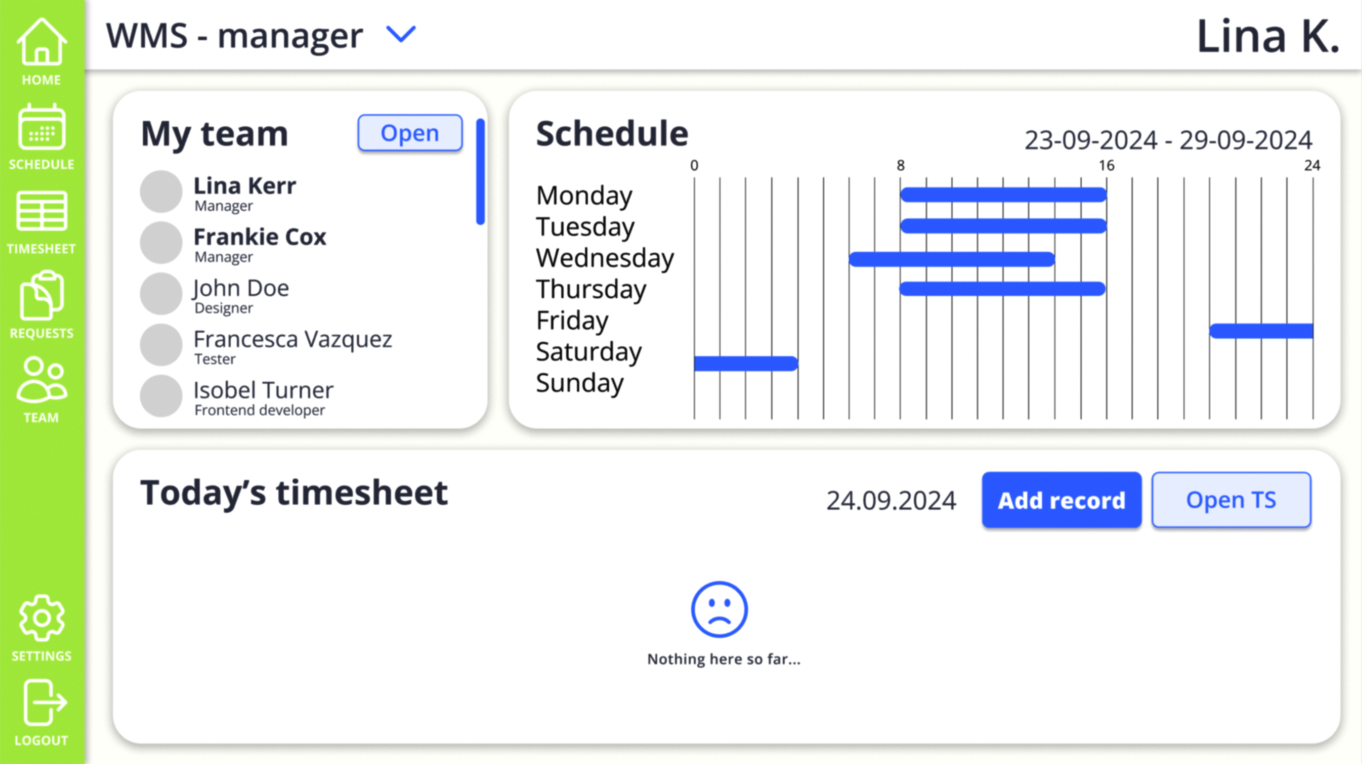
\includegraphics[width=0.8\textwidth, frame]{graf/mainLayout.png}
    \caption{Makieta głównego widoku dla managera}
    \label{fig:mainLayout}
\end{figure}

W całej aplikacji zdecydowano użyć jednolitego kroju bezszeryfowej czcionki \texttt{Open\nolinebreak Sans}, która została zaprojektowana z myślą o czytelności na ekranach. Ta sama myśl przyświecała przy jej wyborze. Pomimo jej silnej inspiracji krojami klasycznymi, posiada nowoczesny charakter i zachowuje czytelność. Elementy nagłówkowe korzystają z jej wersji pogrubionej lub półpogrubionej. Interfejs użytkownika automatycznie dostosowuje wielkość czcionek do preferencji użytkownika.
\newpage
Przy projektowaniu interfejsu skorzystano z podejścia Agile UX - metodologii, która zakłada tworzenie wysokiej jakości produktu w sposób iteracyjny. Stąd też interfejs użytkownika miał kilka wersji, zanim osiągnął obecną formę. Wszystkie zmiany były konsultowane z osobami niezwiązanymi z projektem, aby uzyskać jak największą użyteczność i~zadowolenie użytkowników. Przykład zmian w karcie harmonogramu, na widoku głównym został przedstawiony na rysunku \ref{fig:uxChanges}.

\begin{figure}[H]
    \centering
    \begin{subfigure}[b]{0.49\textwidth}
        \centering
        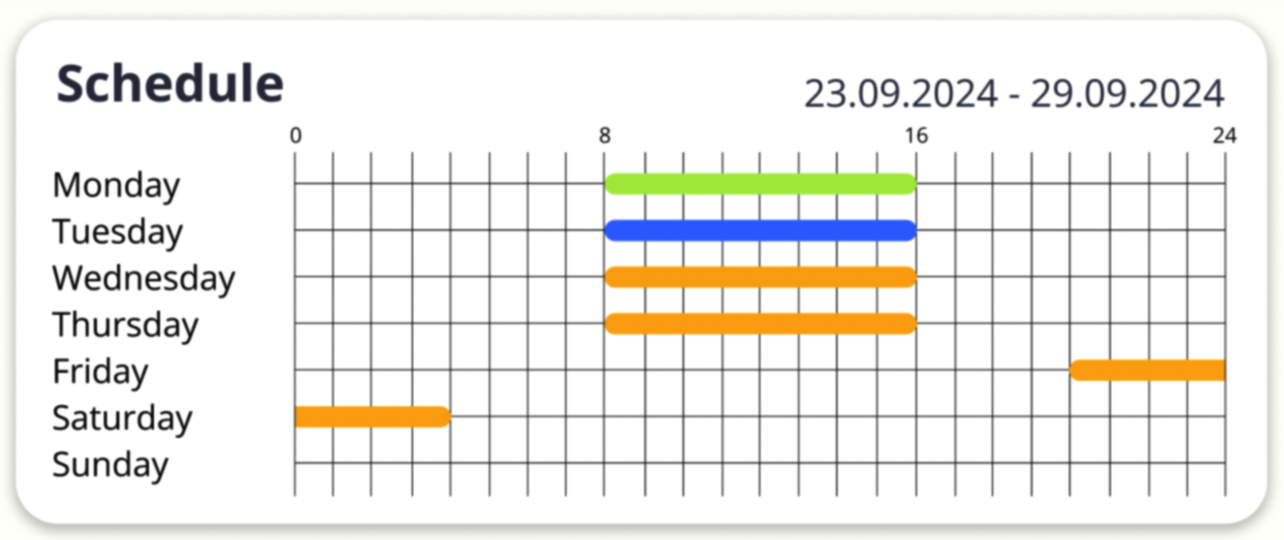
\includegraphics[width=0.9\textwidth, frame]{graf/sch1.png}
        \caption{Wersja pierwotna}
    \end{subfigure}
    \begin{subfigure}[b]{0.49\textwidth}
        \centering
        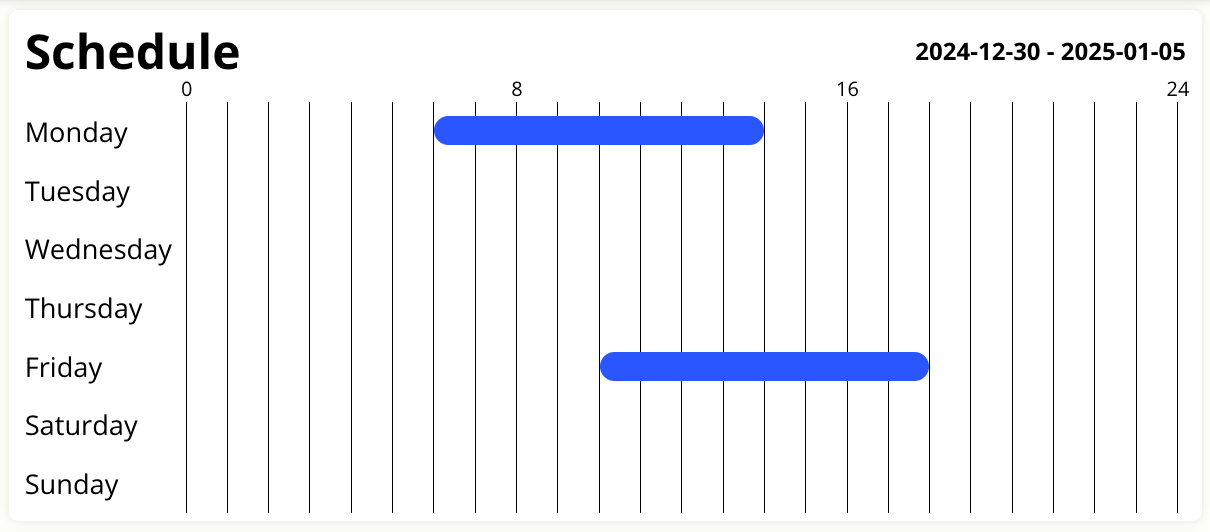
\includegraphics[width=0.9\textwidth, frame]{graf/schE.png}
        \caption{Wersja końcowa}
    \end{subfigure}
    \caption{Zmiany w interfejsie użytkownika}
    \label{fig:uxChanges}
\end{figure}

Pierwsza wersja - mimo, że bogatsza - była uznana za zbyt skomplikowaną i nieczytelną, zwłaszcza jeśli chodzi o użyte kolory. Wersja końcowa została pozbawiona części elementów, uzyskując w zamian bardziej przejrzysty i czytelny interfejs.

\subsection{Kolorystyka}

Przy projektowaniu interfejsu użytkownika zdecydowano się na użycie ciepłych kolorów, które są przyjemne dla oka i nie męczą wzroku. Wśród nich wybrano trzy, które reprezentują poszczególne role w systemie oraz dodają charakteru interfejsowi. Użyto również kilku odcieni do oznaczania elementów informacyjnych. W aplikacji używane są następujące kolory:
\begin{itemize}
    \item \texttt{\#FCAB10} --- pomarańczowy, kolor użytkownika,
    \item \texttt{\#ACE849} --- zielony, kolor managera,
    \item \texttt{\#3772FF} --- niebieski, kolor administratora,
    \item \texttt{\#FFFFFA} --- kolor tła,
    \item \texttt{\#4BB543} --- kolor potwierdzenia,
    \item \texttt{\#DC3545} --- kolor błędu,
    \item \texttt{\#FFC107} --- kolor ostrzeżenia,
    \item \texttt{\#E6EDFF} --- kolor uzupełniający.
\end{itemize}

\subsection{Struktura widoku}

Każdy widok aplikacji dla zalogowanego użytkownika składa się z trzech głównych elementów:
\begin{itemize}
    \item paska nawigacyjnego umieszczonego po lewej stronie ekranu, dzięki któremu użytkownik może szybko i łatwo poruszać się po aplikacji,
    \item górnej belki z skróconą nazwą użytkownika i jego zespołem,
    \item głównego obszaru, w którym wyświetlane są poszczególne karty z informacjami.
\end{itemize}

Makieta struktury widoku została przedstawiona na rysunku \ref{fig:layout}.

\begin{figure}[H]
    \centering
    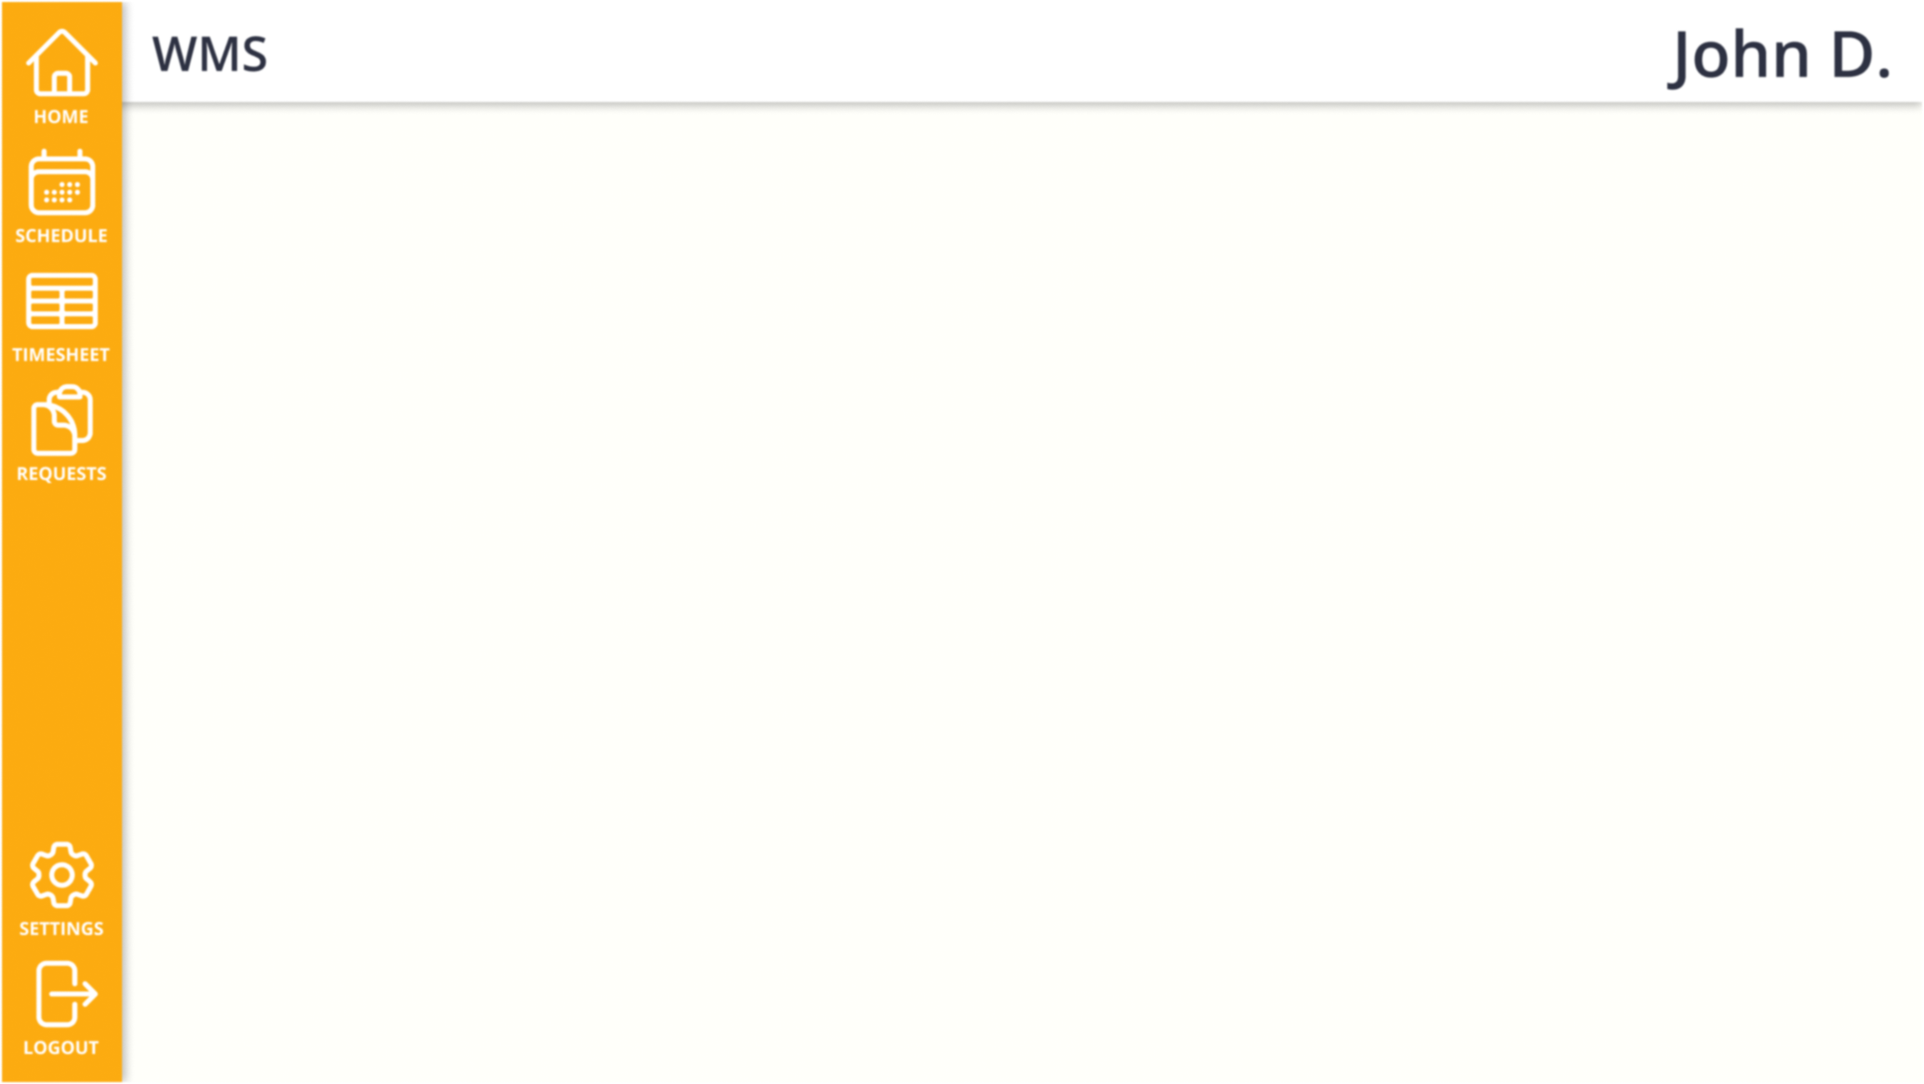
\includegraphics[width=0.8\textwidth, frame]{graf/front/layoutMockup.png}
    \caption{Makieta struktury widoku}
    \label{fig:layout}
\end{figure}

Komponenty są umieszczane na obszarze głównym z wykorzystaniem siatki CSS Grid, o 12 kolumnach i 10 wierszach, dzięki czemu możliwe jest ich łatwe i elastyczne pozycjonowanie na stronie.

\subsection{Strona logowania}

Logowanie do systemu odbywa się poprzez formularz, w którym użytkownik musi podać swoją nazwę użytkownika oraz hasło. W przypadku, gdy użytkownik nie ma jeszcze ustawionego hasła pojawi się dodatkowe pole. Użytkownik musi potwierdzić wcześniej wpisane hasło, a to - jeżeli jest zgodne - zostanie zapamiętane w systemie. Wszelkie błędy związane z logowaniem są wyświetlane w formie komunikatów pod polami formularza.
Widok strony logowania został przedstawiony na rysunku \ref{fig:loginPage}.

\begin{figure}[H]
    \centering
    
\includegraphics[width=0.8\textwidth, frame]{graf/front/loginPage.png}
    \caption{Widok strony logowania}
    \label{fig:loginPage}
\end{figure}

\subsection{Panel główny}

Panel główny jest pierwszym widokiem, który widzi zalogowany użytkownik. Przy projektowaniu zdecydowano, że na panelu głównym znajdą się informacje, które użytkownik będzie najczęściej potrzebował. W związku z tym umieszczono na nim skład aktualnego zespołu, harmonogram pracy w bieżącym tygodniu, oraz szybki dostęp do karty pracy w~danym dniu. Przykładowy panel użytkownika został przedstawiony na rysunku \ref{fig:userDashboard}.

\begin{figure}[H]
    \centering
    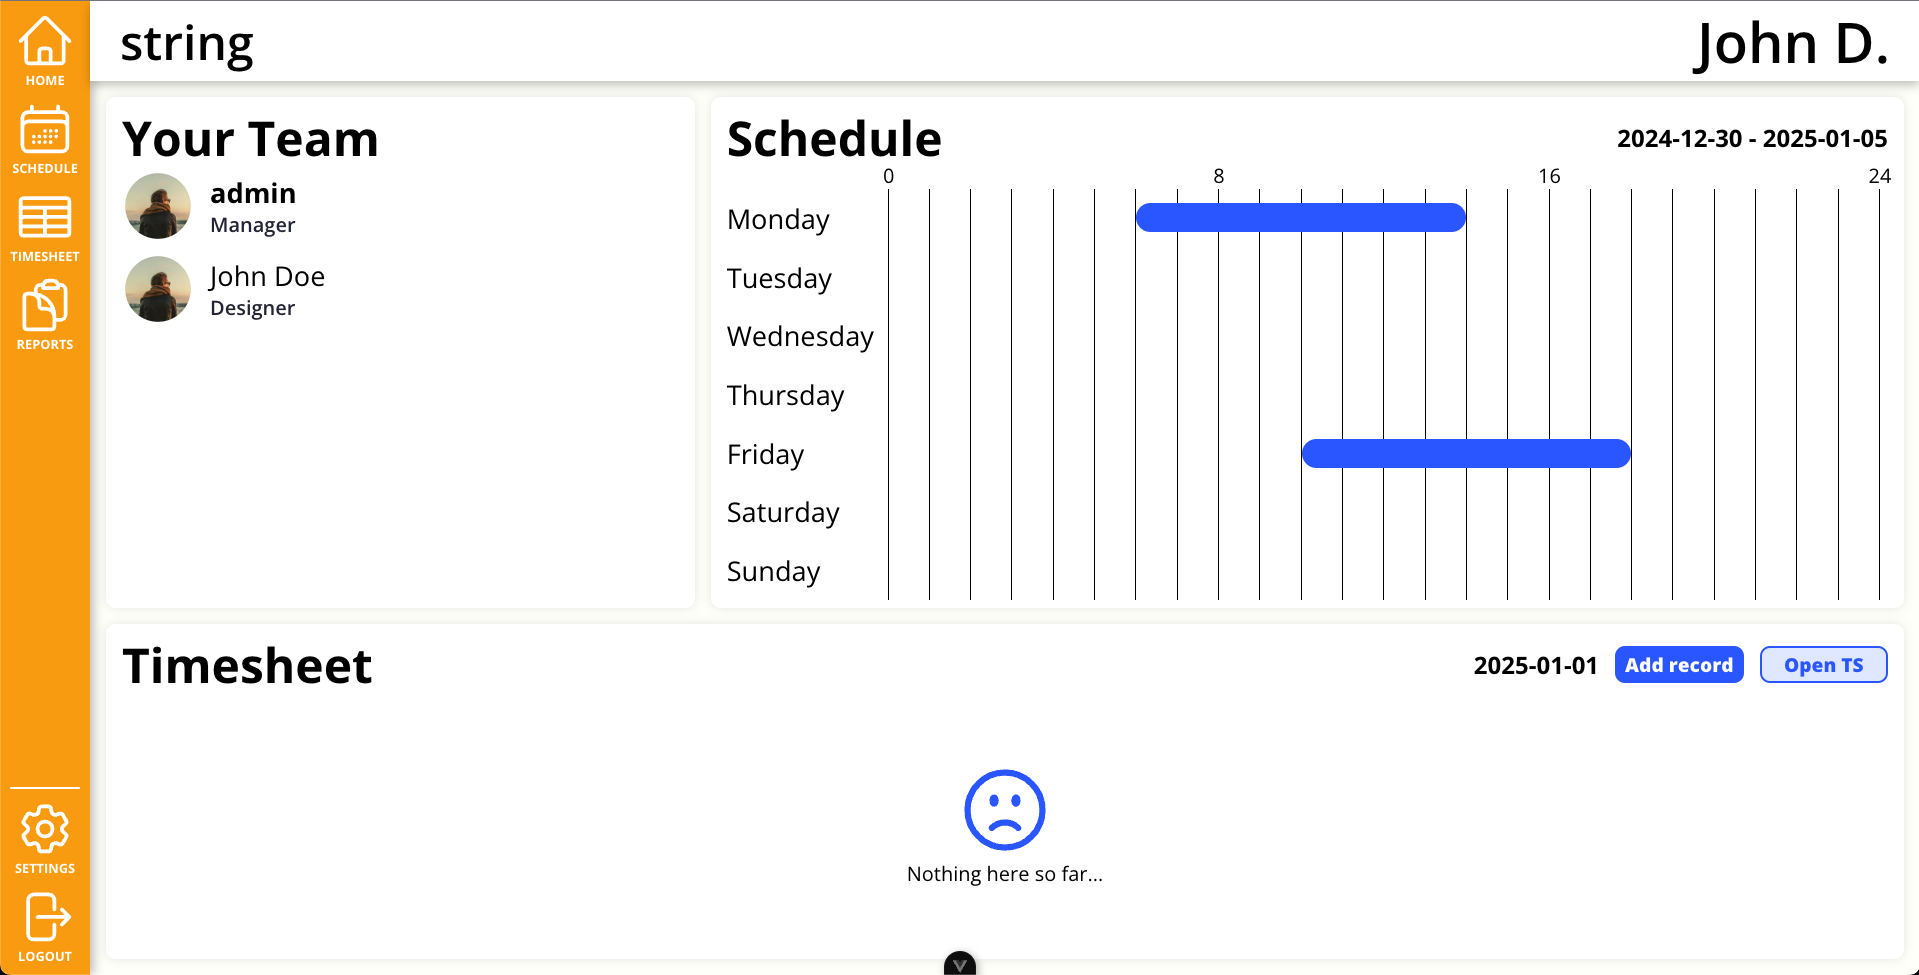
\includegraphics[width=0.8\textwidth, frame]{graf/userDashboard.png}
    \caption{Panel użytkownika}
    \label{fig:userDashboard}
\end{figure}

\subsection{Widok użytkowników}

Po przejściu do widoku użytkowników, administratorowi wyświetlana jest lista wszystkich kont zarejestrowanych w systemie. Istnieje możliwość filtrowania wyników wpisując dane użytkownika w pole wyszukiwania. W tabeli znajdują się skrócone informacje o~użytkowniku, przedostatnia kolumna przedstawia aktualną rolę użytkownika, a ostatnia kolumna umożliwia wykonywanie akcji otwarcia szczegółów, edycji, archiwizacji oraz usunięcia konta. Widoczność poszczególnych akcji zależy od statusu danego konta i jest ustalana przez serwer. Widok użytkowników został przedstawiony na rysunku \ref{fig:usersView}. Kliknięcie w ikony akcji otwiera odpowiednie okno dialogowe, szufladę lub wykonuje ją bezpośrednio. Akcje krytyczne z punktu widzenia bezpieczeństwa, wymagają potwierdzenia w osobnym oknie dialogowym.

\begin{figure}[H]
    \centering
    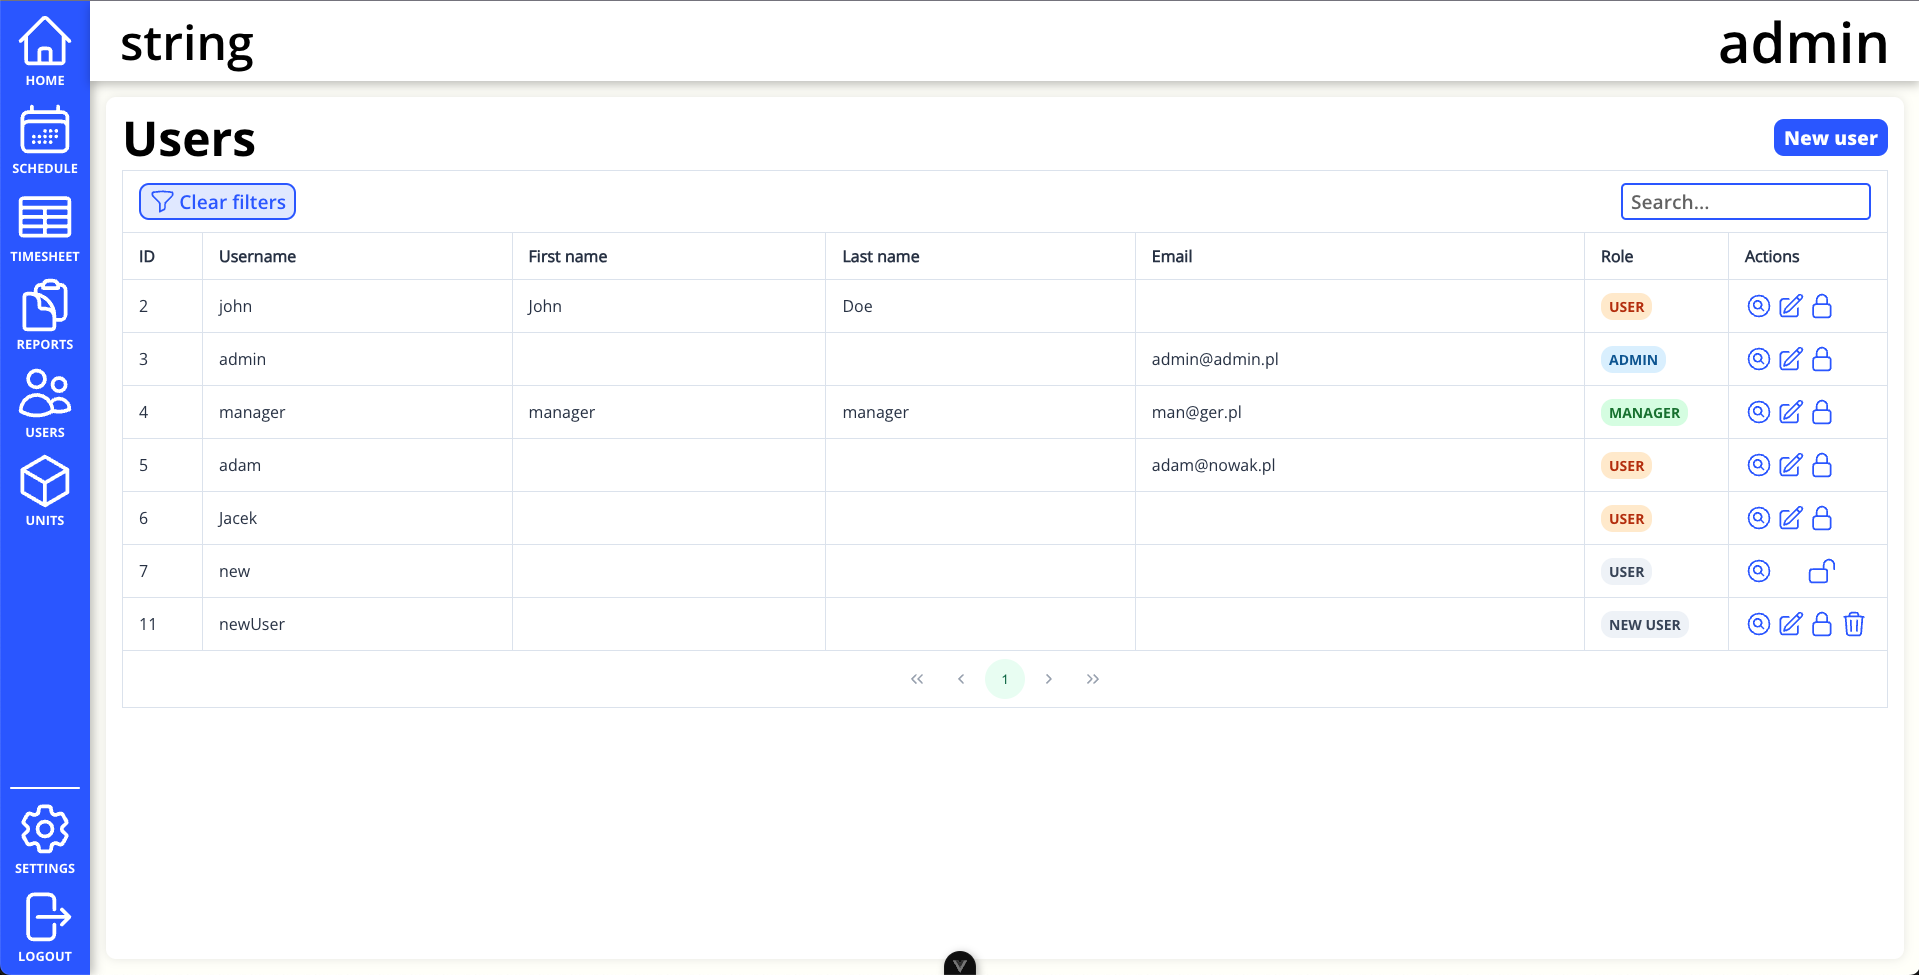
\includegraphics[width=0.8\textwidth, frame]{graf/front/users.png}
    \caption{Widok użytkowników}
    \label{fig:usersView}
\end{figure}

Otwarcie widoku edycji użytkownika umożliwia zmianę jego danych. Obowiązkowe pola są oznaczone gwiazdką, a przesłanie formularza z niepoprawnymi danymi skutkuje wyświetleniem komunikatu o błędzie. W przypadku poprawnego przesłania formularza, użytkownik zostaje poinformowany o sukcesie operacji, okno dialogowe zamyka się, a~tabela użytkowników jest odświeżana.

\begin{figure}[H]
    \centering
    \begin{subfigure}[b]{0.49\textwidth}
        \centering
        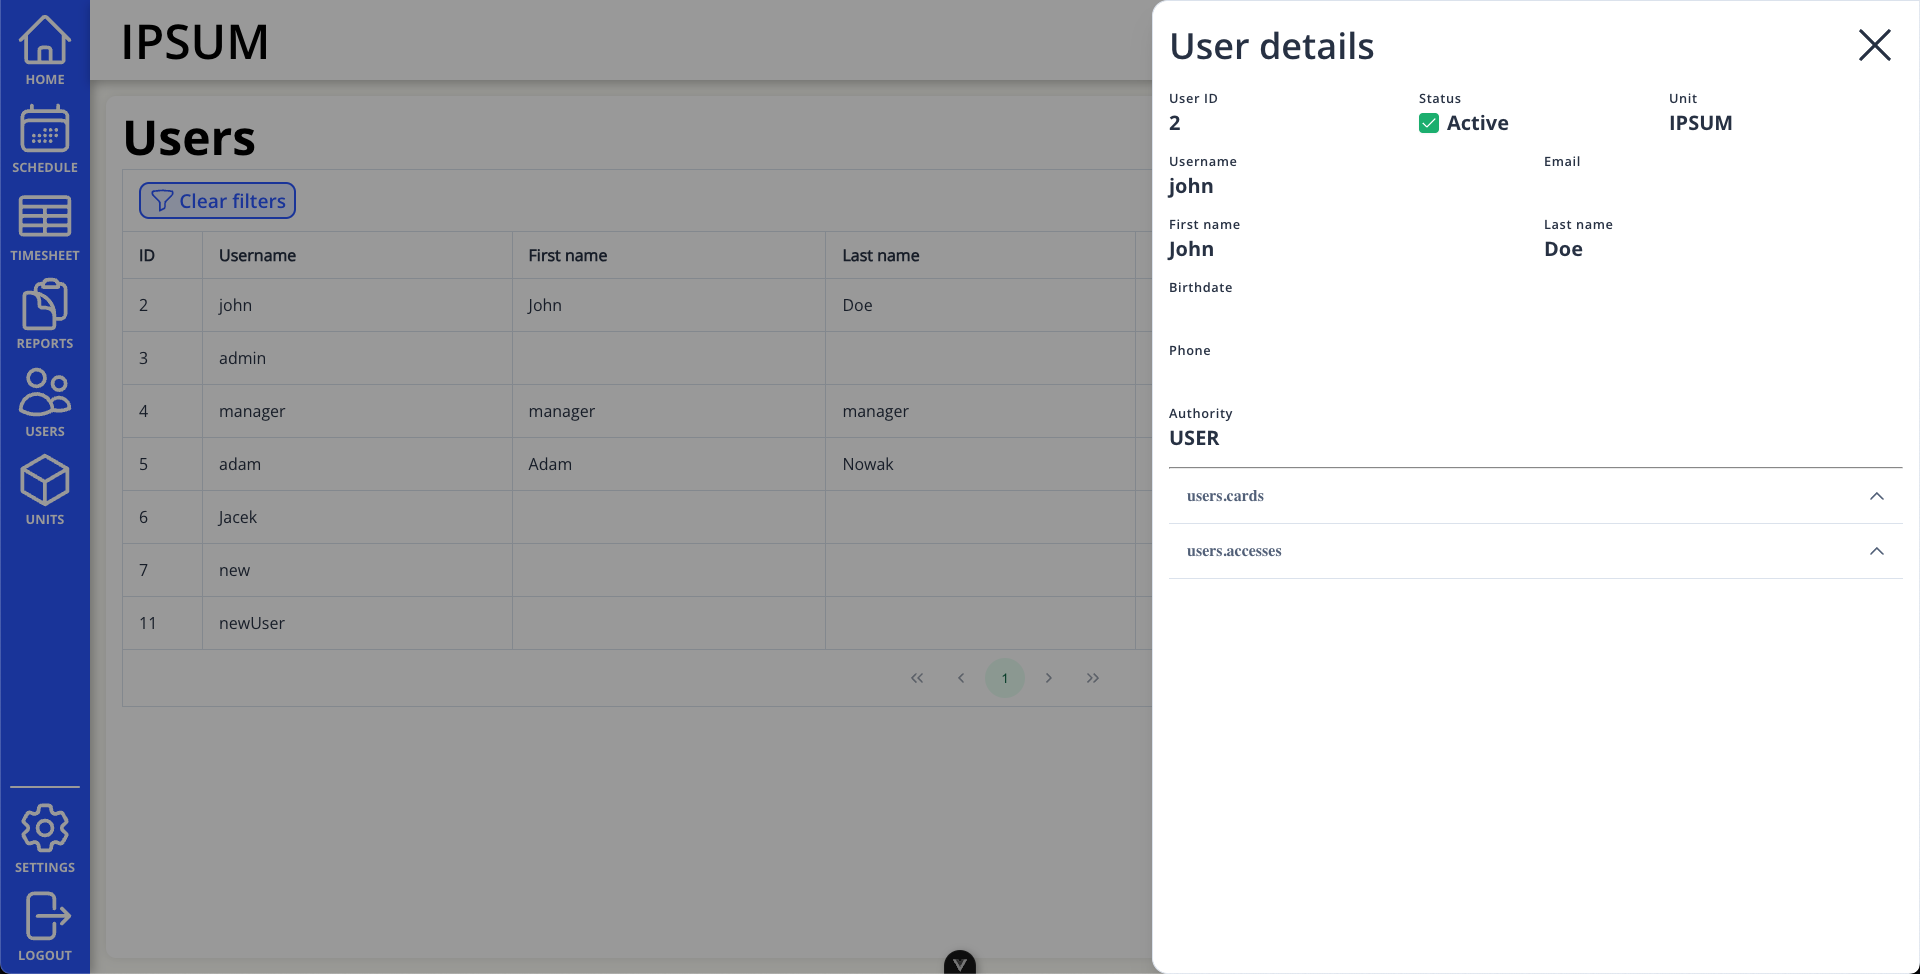
\includegraphics[width=0.8\textwidth, frame]{graf/front/userDetails.png}
        \caption{Szczegóły użytkownika}
    \end{subfigure}
    \begin{subfigure}[b]{0.49\textwidth}
        \centering
        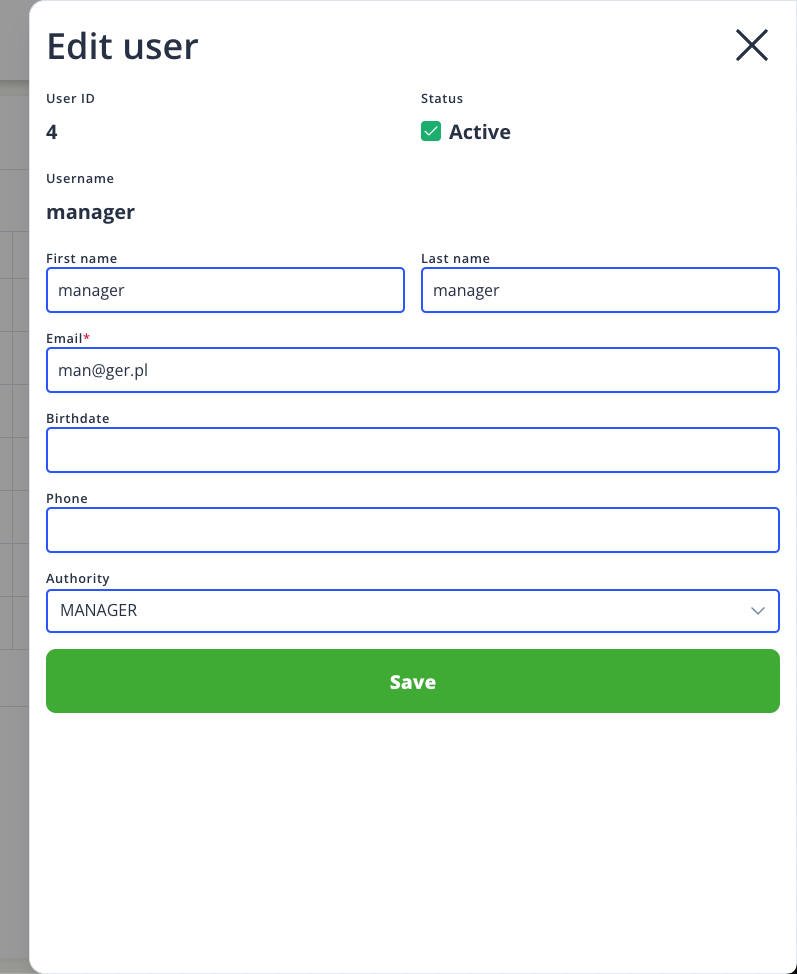
\includegraphics[width=0.8\textwidth, frame]{graf/front/editUser.png}
        \caption{Edycja użytkownika}
    \end{subfigure}
    \caption{Okna dialogowe widoku użytkowników}
    \label{fig:userDialogs}
\end{figure}

\subsection{Widok karty pracy}

Widok karty pracy rozszerza funkcjonalności karty z panelu głównego. Oprócz możliwości dodawania wpisów, użytkownik może przeglądać swoje wpisy z wybranego przez siebie zakresu czasu. Informacje są sortowane zgodnie z chronologią ich dodawania. Wspomniany widok został przedstawiony na rysunku \ref{fig:timesheetView}. Dodawanie wpisów odbywa się poprzez formularz otwierany w oknie dialogowym po kliknięciu odpowiedniego przycisku. Został on ukazany na rysunku \ref{fig:timesheetDialog}.

\begin{figure}[H]
    \centering
    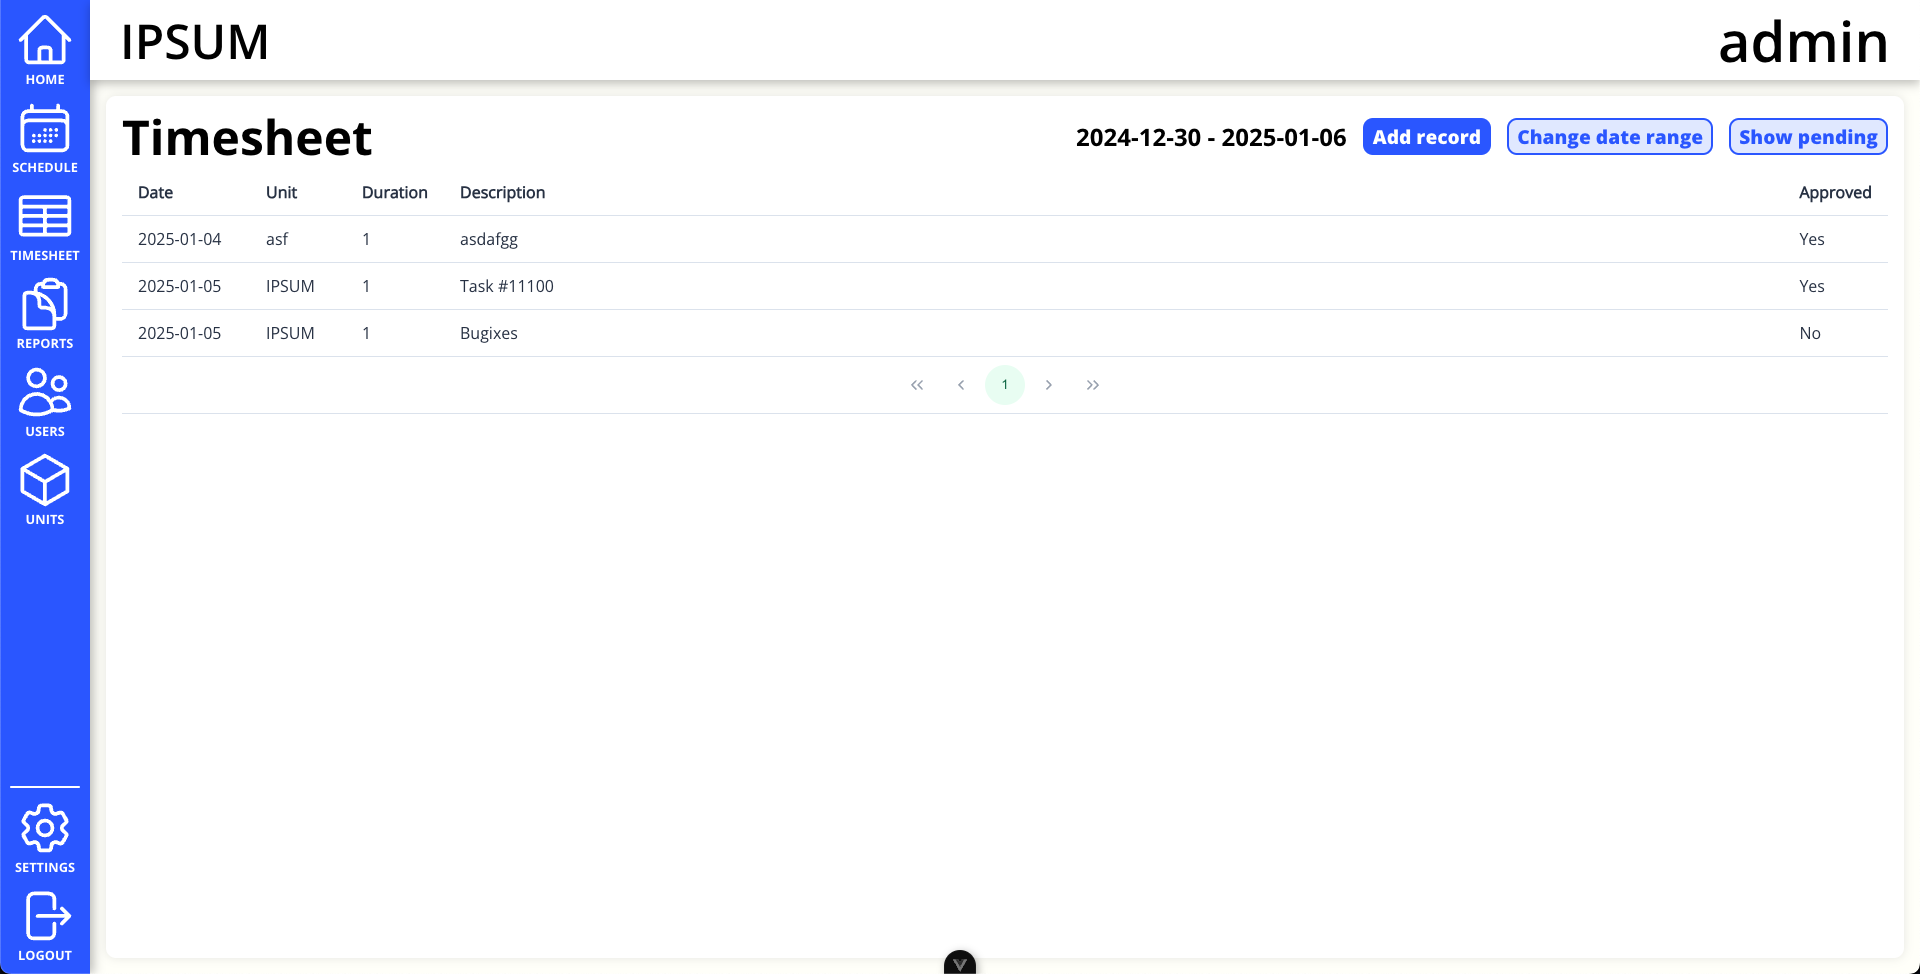
\includegraphics[width=0.8\textwidth, frame]{graf/front/timesheet.png}
    \caption{Widok karty pracy}
    \label{fig:timesheetView}
\end{figure}

\begin{figure}[H]
    \centering
    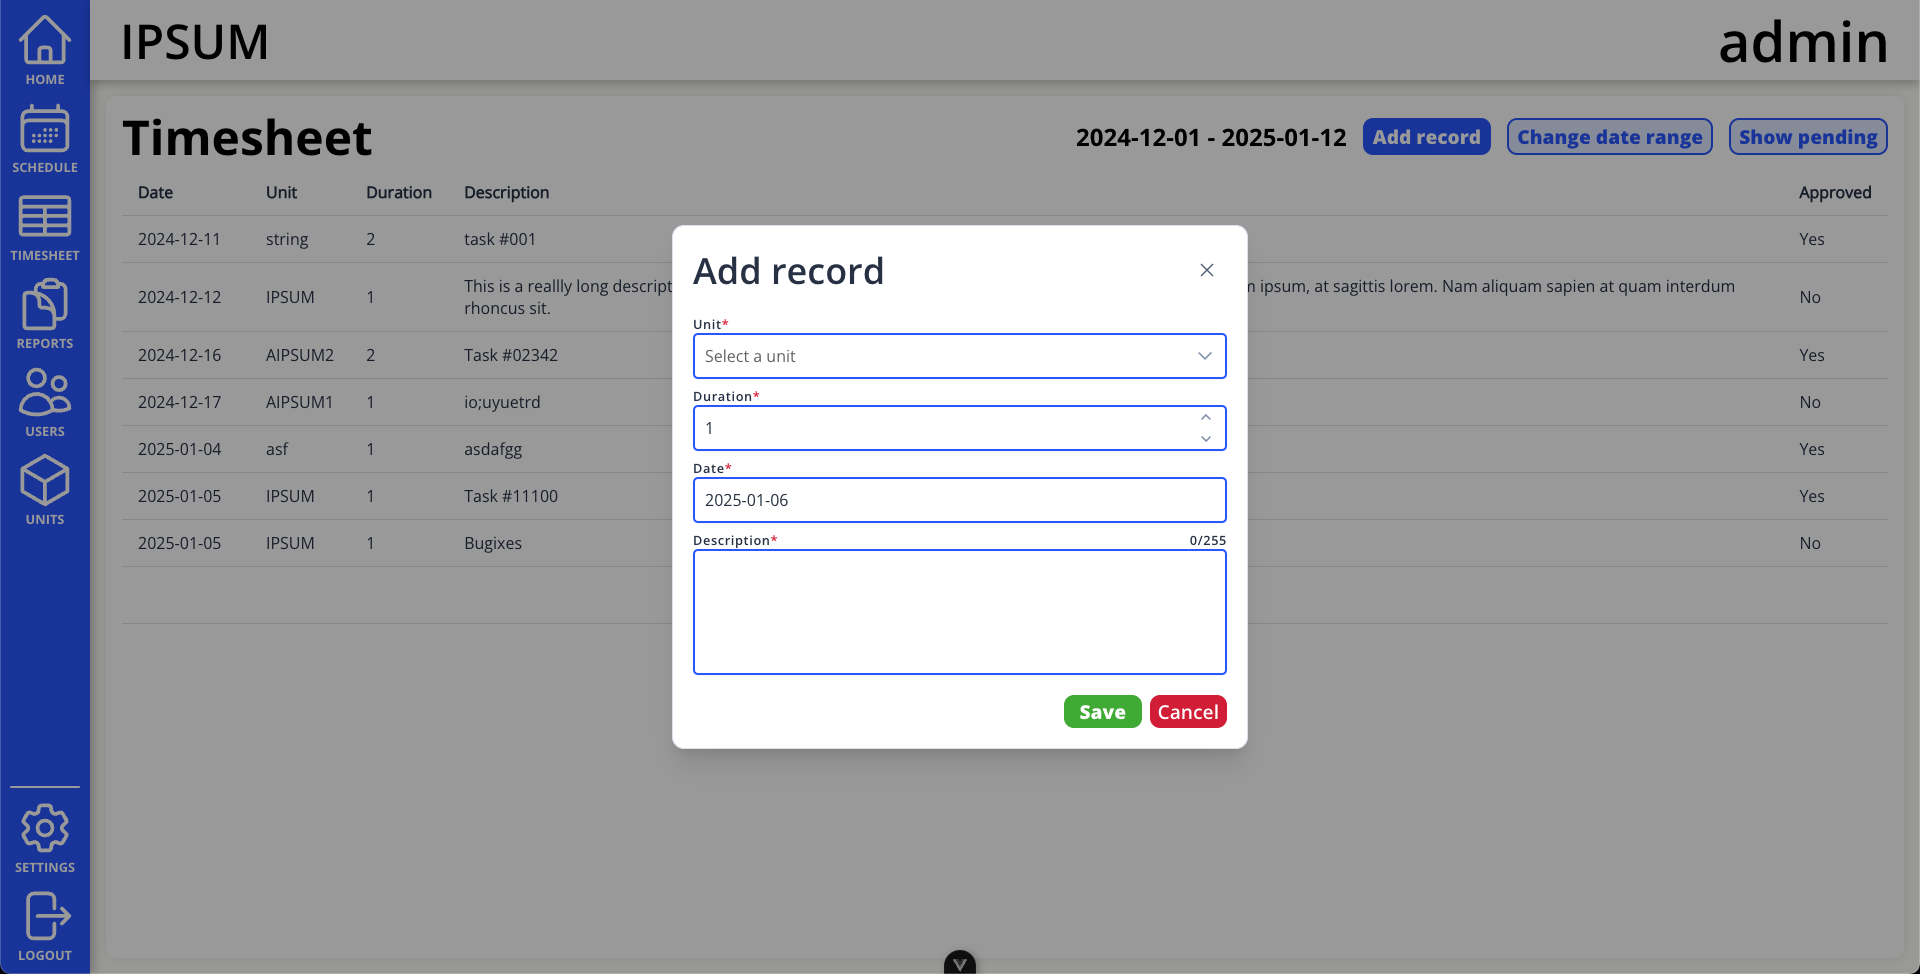
\includegraphics[width=0.5\textwidth]{graf/front/timesheetAddRecord.png}
    \caption{Okno dialogowe dodawania wpisu do karty pracy}
    \label{fig:timesheetDialog}
\end{figure}

Administratorzy i managerowie mają możliwość przejścia do widoku wpisów oczekujących na akceptację. Mogą z tego miejsca ręcznie zatwierdzać lub odrzucać wpisy, lub~automatycznie zaakceptować wszystkie z nich. W zależności od statusu wpisu, w tabeli kart pracy pojawiają się odpowiednie oznaczenia. Widok wpisów oczekujących na akceptację został przedstawiony na rysunku \ref{fig:timesheetApprovalView}.

\begin{figure}[H]
    \centering
    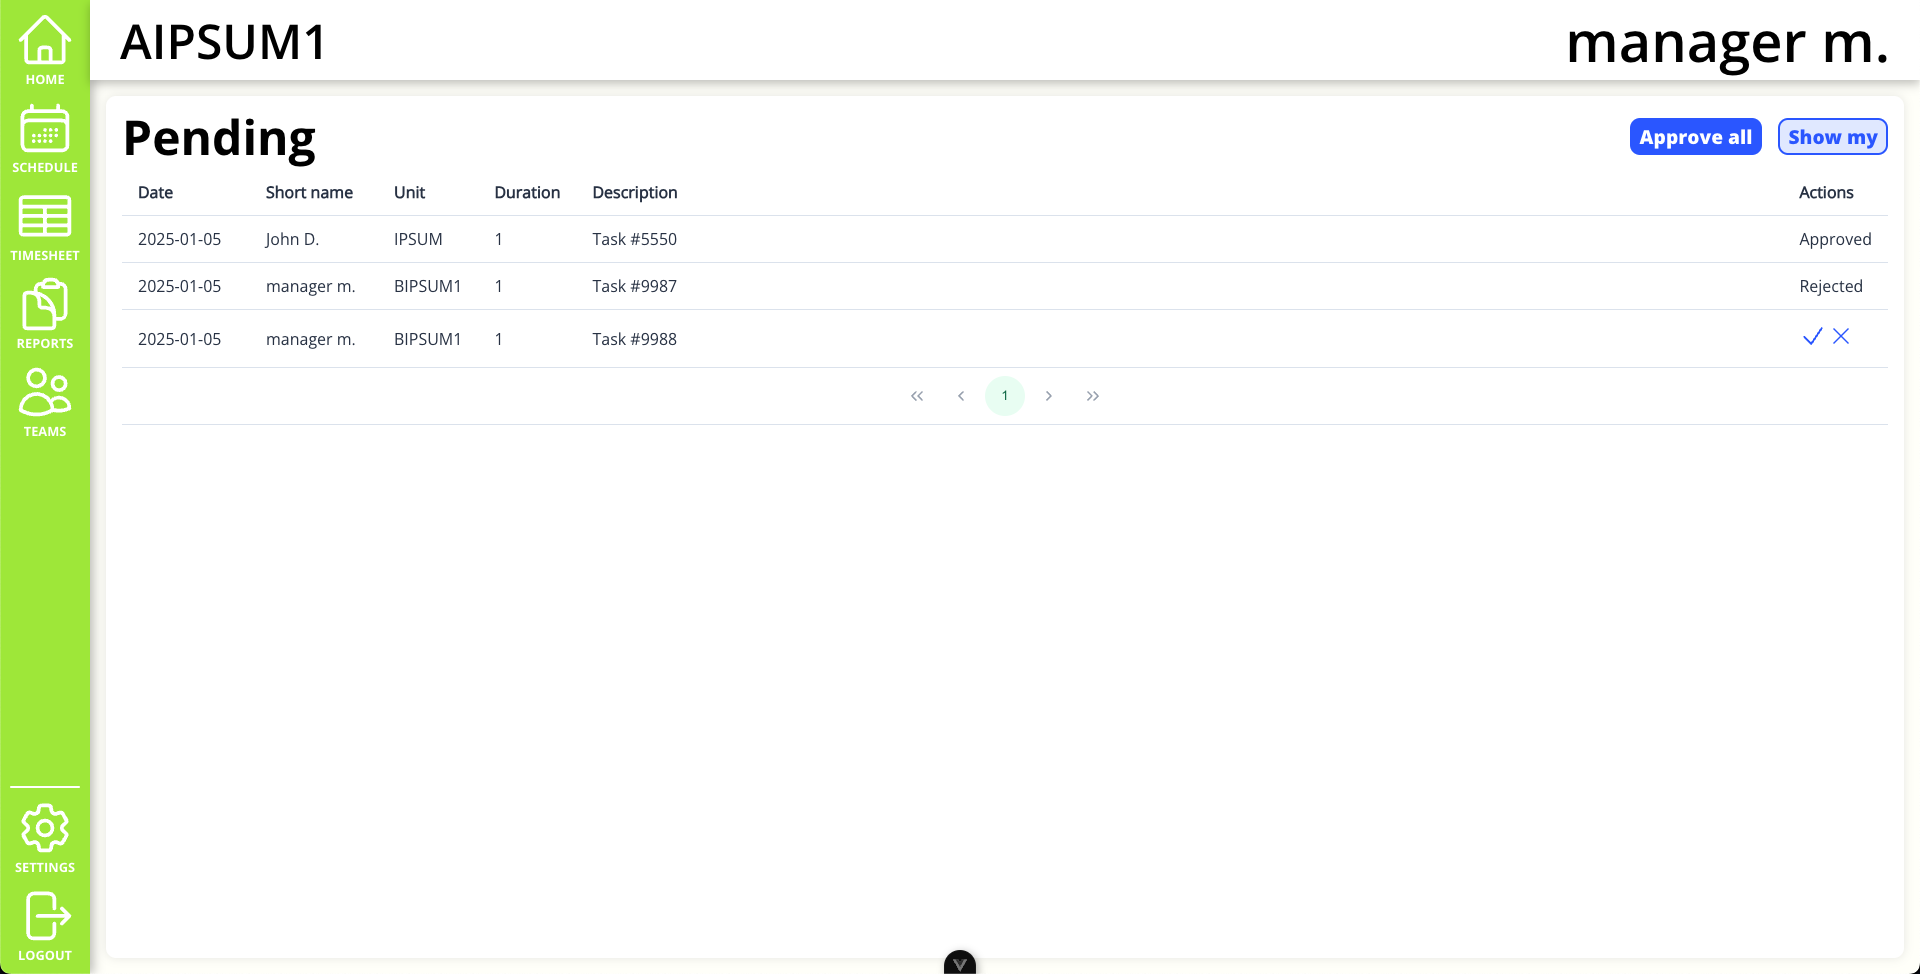
\includegraphics[width=0.8\textwidth, frame]{graf/front/timesheetManagerPending.png}
    \caption{Widok wpisów oczekujących na akceptację}
    \label{fig:timesheetApprovalView}
\end{figure}


\subsection{Widok jednostek organizacyjnych}

Widok został skonstruowany w taki sposób, aby nie ukazywać wszystkich informacji na raz. Hierarchiczna struktura jednostek organizacyjnych skutkuje wyświetleniem jedynie tych, które są bezpośrednio zależne od wybranej jednostki. Te, które wyświetlają się zaraz po przejściu do widoku nie posiadają żadnych jednostek nadrzędnych. Przejście do podjednostek odbywa się poprzez kliknięcie w odpowiednią ikonę w kolumnie akcji. Przejście do wyższego poziomu jest możliwe klikając nazwę jednostki w nagłówku karty. Widok jednostek organizacyjnych przedstawiono na rysunku \ref{fig:unitsView}.

\begin{figure}[H]
    \centering
    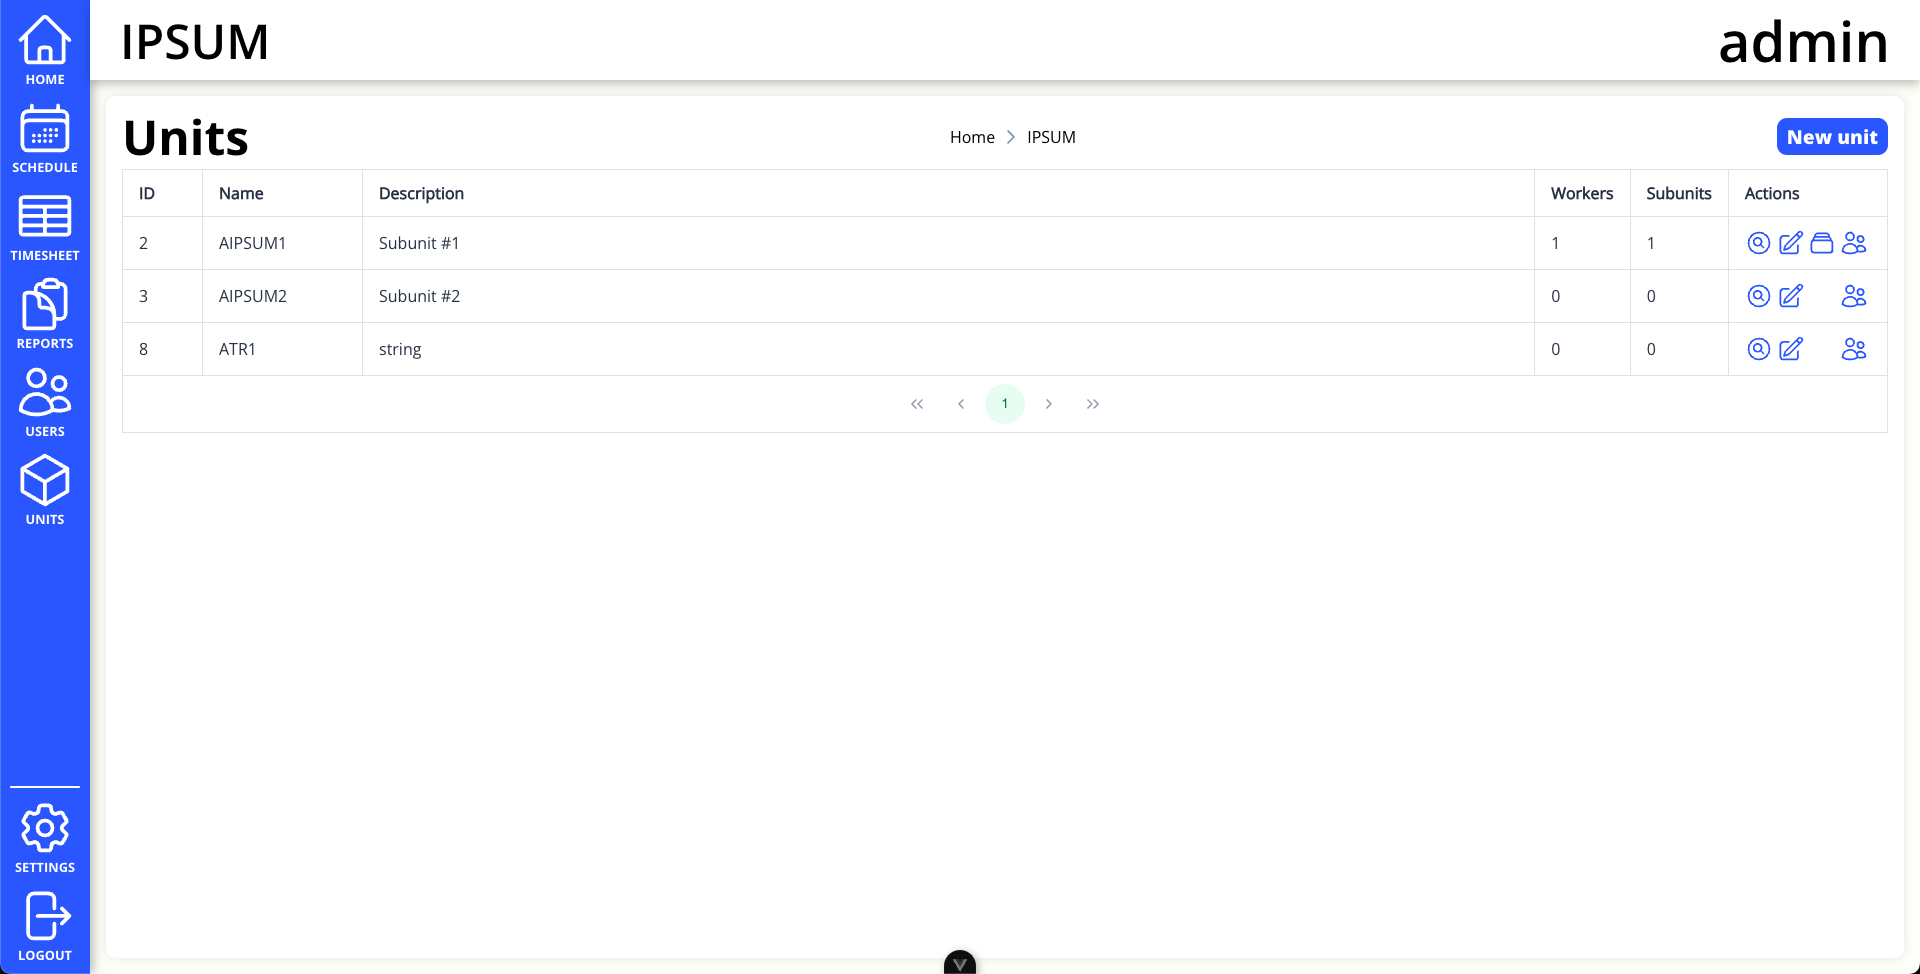
\includegraphics[width=0.8\textwidth, frame]{graf/front/units.png}
    \caption{Widok jednostek organizacyjnych}
    \label{fig:unitsView}
\end{figure}

Kolumna akcji może zawierać maksymalnie cztery ikony: otwarcie szczegółów, edycję, przejście do podjednostek oraz otwarcie widoku pracowników (rys. \ref{fig:unitDialogs}). Ostatnia z akcji umożliwia przeglądanie użytkowników pracujących w danej jednostce wraz z ich rolami. W przypadku braku pracowników, tabela jest pusta. Kliknięcie przycisku w górnej części szuflady otwiera okno dialogowe, w którym możliwe jest dodanie nowych użytkowników do jednostki. Po wybraniu użytkowników aplikacja prosi o nadanie ról, a następnie dodaje ich do jednostki. Po zakończeniu operacji okno dialogowe zamyka się, a tabela jest odświeżana. Otwierane okna są ukazane na rysunku \ref{fig:unitDialogs2}.

\begin{figure}[H]
    \centering
    \begin{subfigure}[b]{0.49\textwidth}
        \centering
        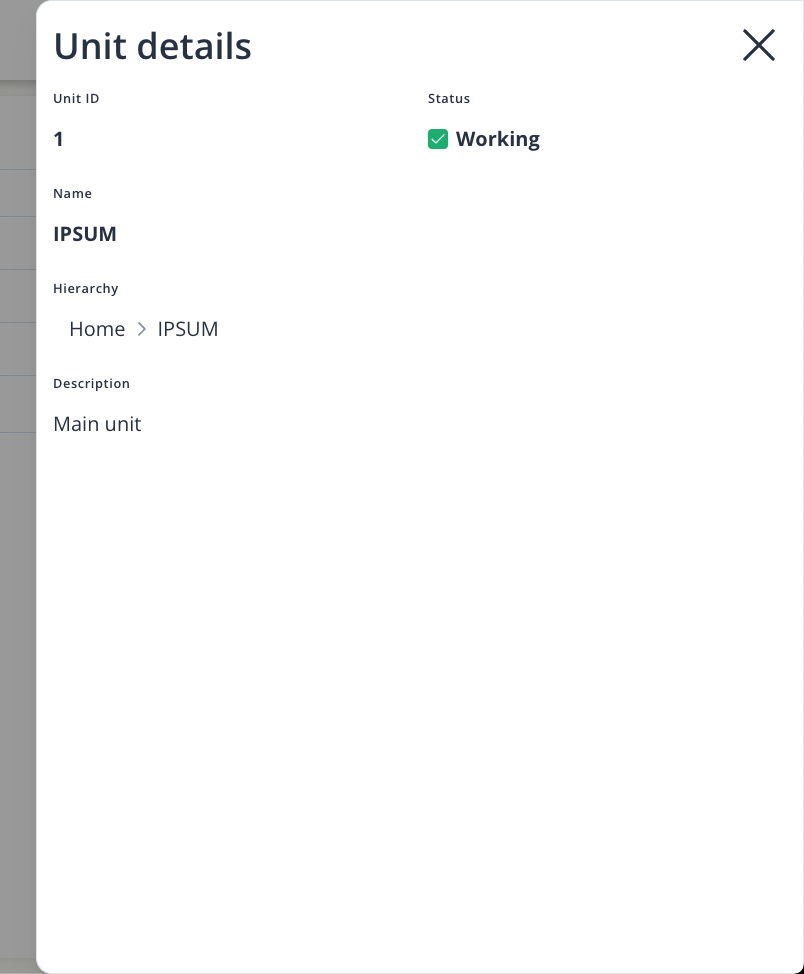
\includegraphics[width=0.8\textwidth, frame]{graf/front/unitDetails.png}
        \caption{Szczegóły jednostki organizacyjnej}
    \end{subfigure}
    \begin{subfigure}[b]{0.49\textwidth}
        \centering
        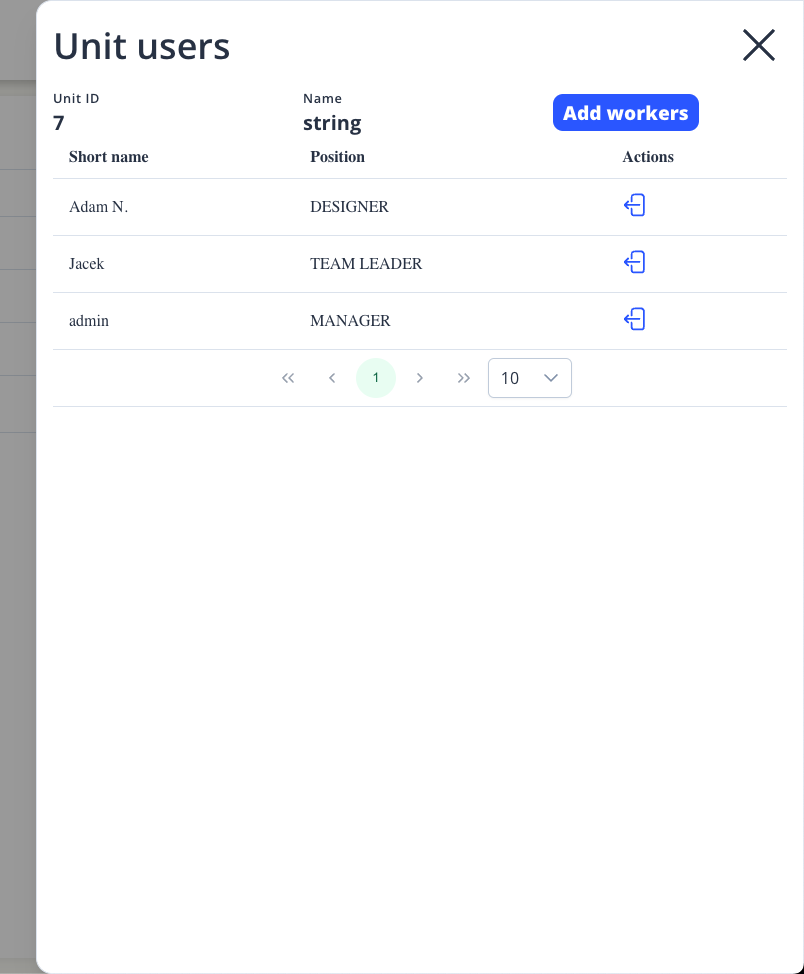
\includegraphics[width=0.8\textwidth, frame]{graf/front/unitWorkers.png}
        \caption{Pracownicy jednostki organizacyjnej}
    \end{subfigure}
    \begin{subfigure}[b]{0.7\textwidth}
        \centering
        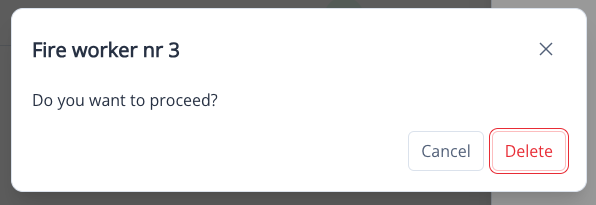
\includegraphics[width=0.8\textwidth, frame]{graf/front/confirmWorkerDelete.png}
        \caption{Potwierdzenie usunięcia użytkownika}
    \end{subfigure}
    \caption{Okna dialogowe widoku jednostek organizacyjnych}
    \label{fig:unitDialogs}
\end{figure}

\begin{figure}[H]
    \centering
    \begin{subfigure}[b]{0.49\textwidth}
        \centering
        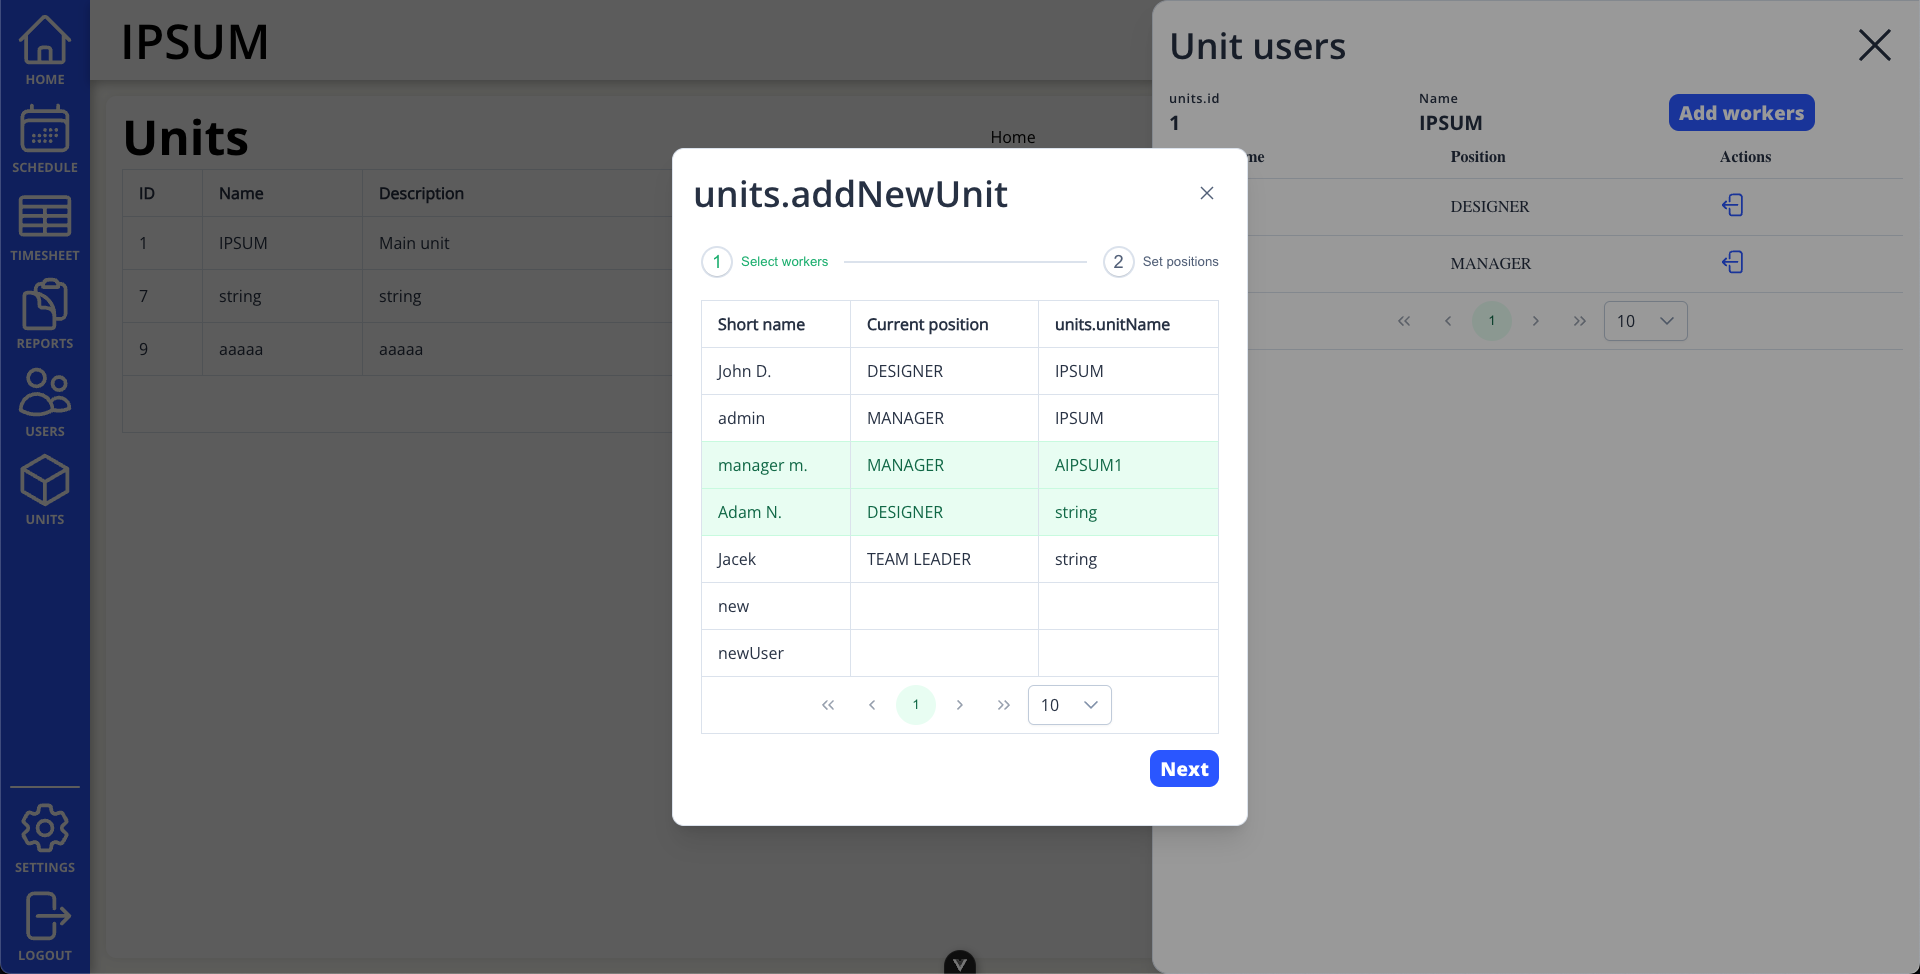
\includegraphics[width=0.8\textwidth]{graf/front/selectWorkers.png}
        \caption{Wybór pracowników}
    \end{subfigure}
    \begin{subfigure}[b]{0.49\textwidth}
        \centering
        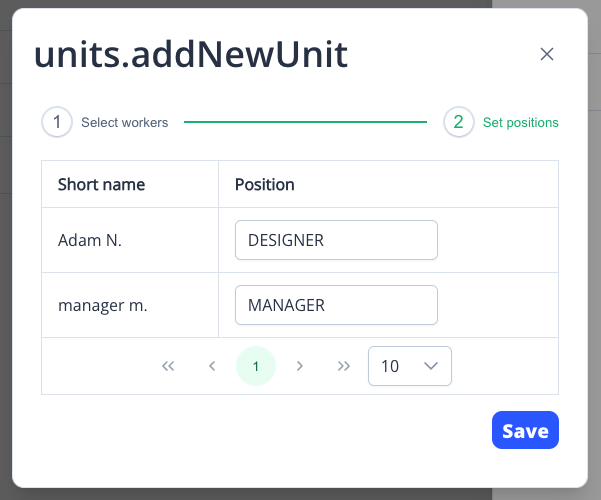
\includegraphics[width=0.8\textwidth]{graf/front/setPositions.png}
        \caption{Ustawienie ról}
    \end{subfigure}
    \caption{Okna dialogowe dodawania użytkowników do jednostki organizacyjnej}
    \label{fig:unitDialogs2}
\end{figure}

\subsection{Widok harmonogramu}

Widok harmonogramu jest rozszerzoną wersją karty z panelu głównego. Użytkownik może przeglądać harmonogram swój oraz swojego zespołu. Wyświetlany jest w formie siatki, na której umieszczane są bloki reprezentujące poszczególne zadania. Są one przypisane do konkretnych dni i godzin, co umożliwia ich łatwe odczytanie. Dodatkowo, każdy z nich posiada informacje o godzinach rozpoczęcia i zakończenia pracy oraz nazwę zespołu. Widok harmonogramu użytkownika został przedstawiony na rysunku \ref{fig:scheduleView}.

\begin{figure}[H]
    \centering
    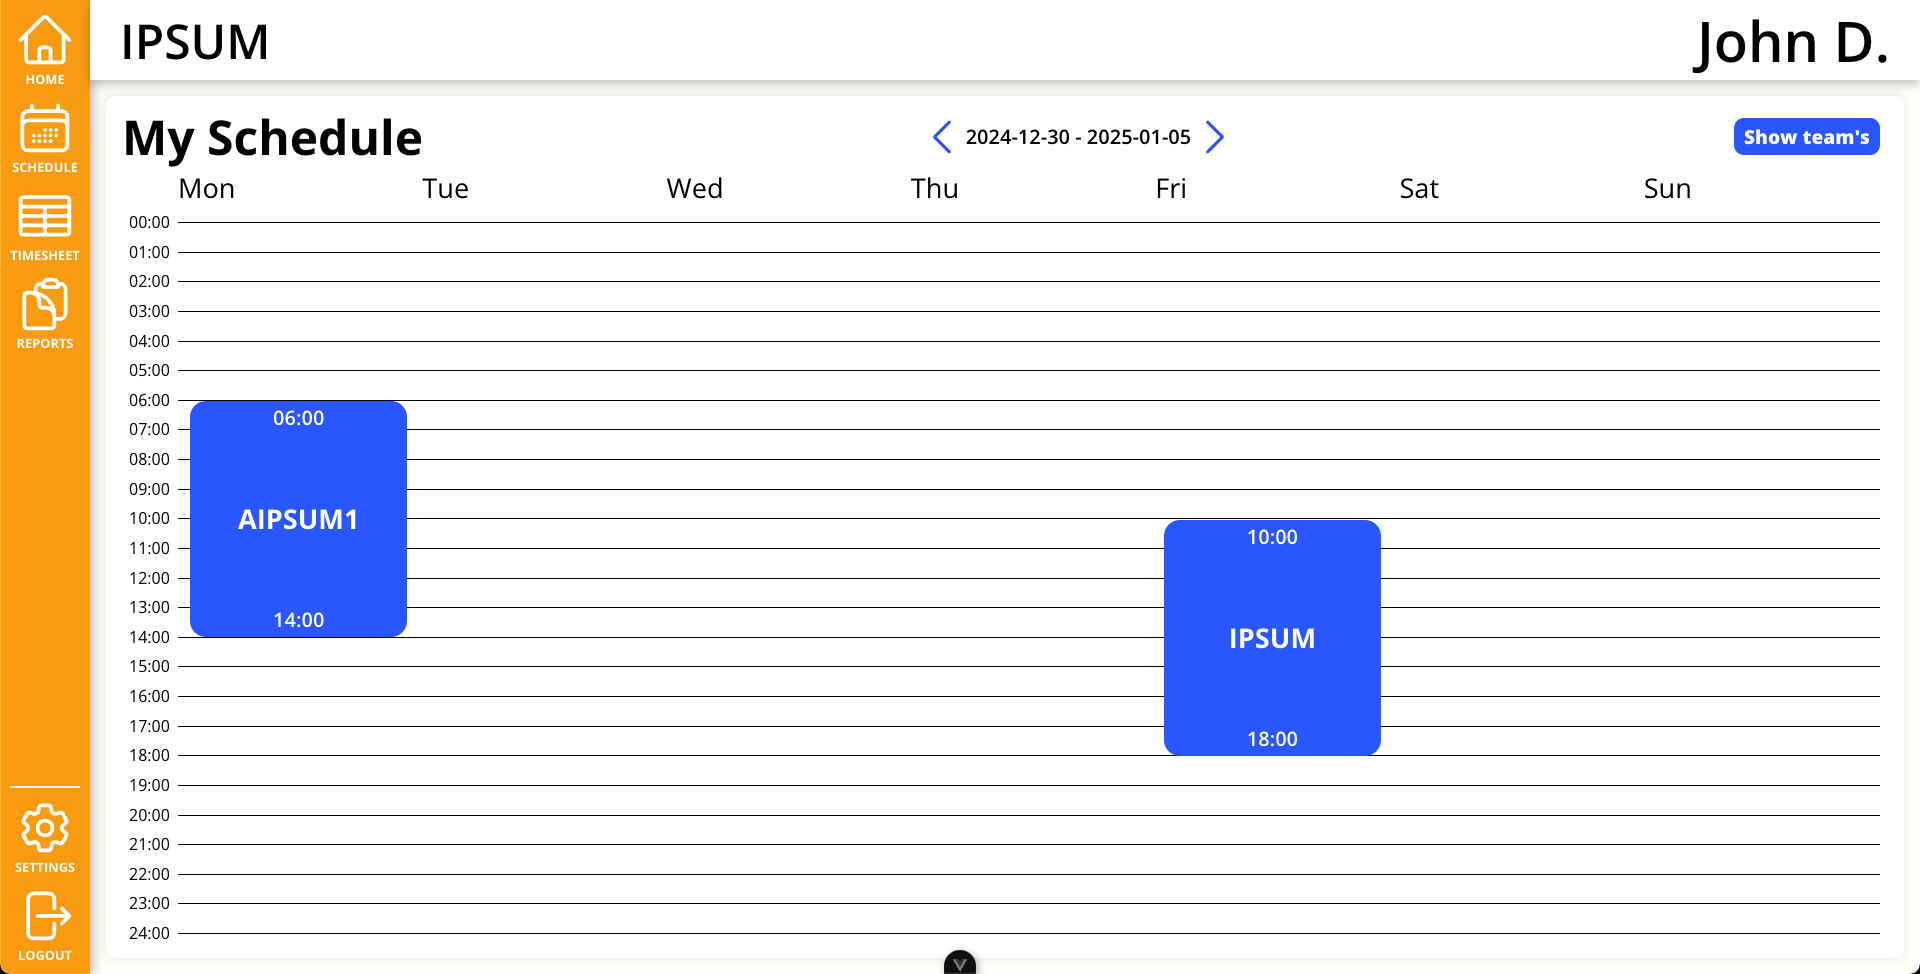
\includegraphics[width=0.8\textwidth, frame]{graf/front/schedule.png}
    \caption{Widok harmonogramu}
    \label{fig:scheduleView}
\end{figure}

Administratorzy oraz managerowie mają możliwość podglądu harmonogramu użytkowników należących do ich zespołu. Odbywa się to poprzez wybór odpowiedniego użytkownika z dodatkowej karty wyświetlanej po prawej stronie widoku. Ikony kół zębatych umożliwiają edycję harmonogramu. Widok harmonogramu użytkownika przed administratora został przedstawiony na rysunku \ref{fig:scheduleManagerView}.

\begin{figure}[H]
    \centering
    \includegraphics[width=0.8\textwidth, frame]{graf/front/userSchedule.png}
    \caption{Widok harmonogramu dla managera}
    \label{fig:scheduleManagerView}
\end{figure}

\subsection{Widok dodawania karty}

Karty zbliżeniowe może dodawać administrator wyłącznie za pomocą aplikacji mobilnej. Po przejściu do odpowiedniej zakładki użytkownik musi zeskanować kartę, a następnie aplikacja wysyła do serwera zapytanie na jej temat. Widok jest różny w zależności od tego, czy karta jest już przypisana do użytkownika, czy nie. Jeżeli w urządzeniu jest wyłączona funkcja NFC (ang. \english{Near Field Communication}), aplikacja wyświetla komunikat o konieczności jej włączenia ukazany na rysunku \ref{fig:cardNFC}. Widoki zostały przedstawione na~rysunkach~\ref{fig:cardView}.

\begin{figure}[H]
    \centering
    \begin{subfigure}[b]{0.3\textwidth}
        \centering
        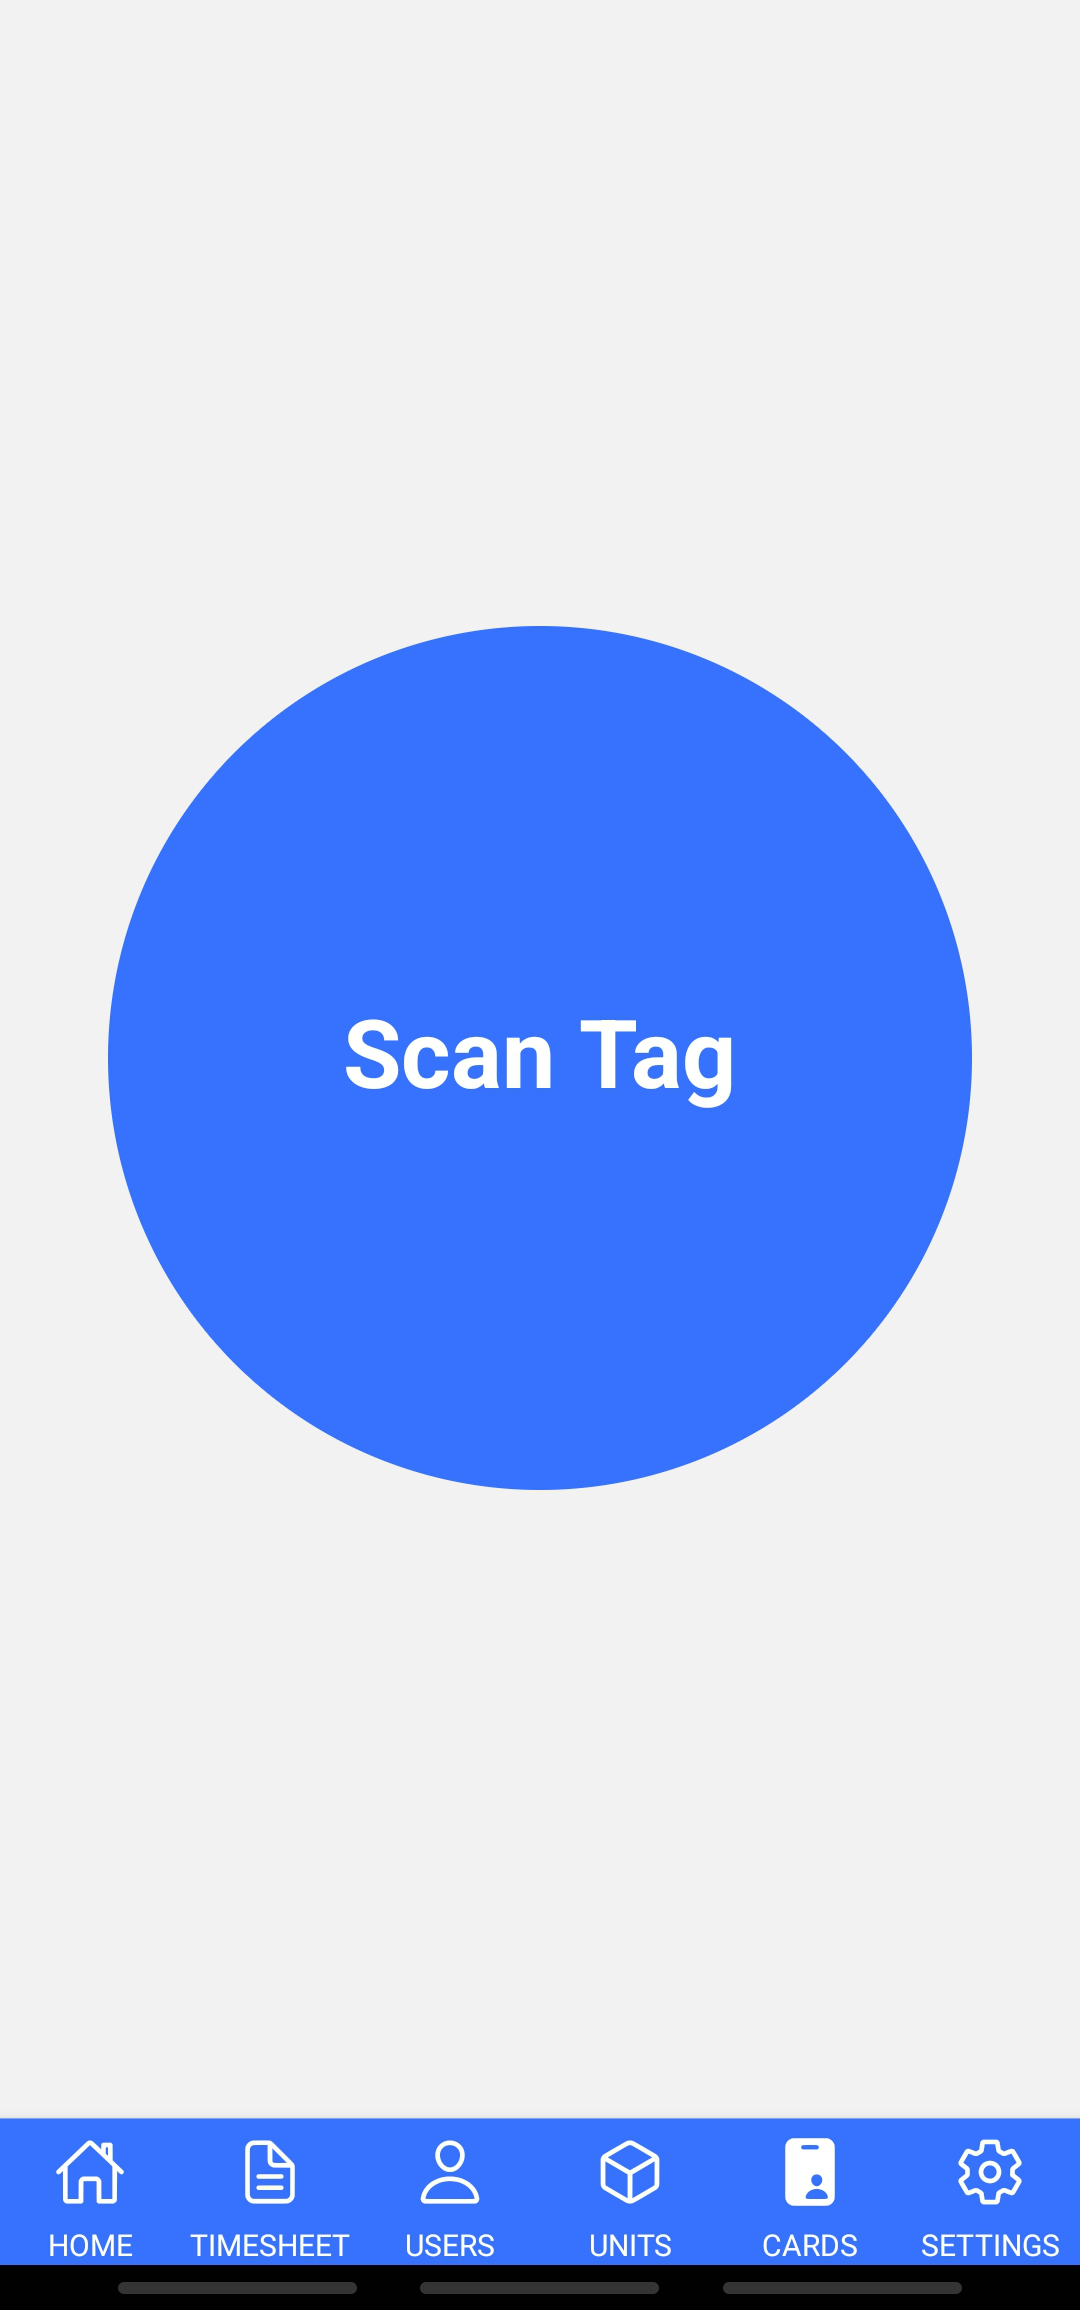
\includegraphics[width=\textwidth, frame]{graf/mobile/cardView.jpg}
        \caption{Skanowanie}
    \end{subfigure}
    \begin{subfigure}[b]{0.3\textwidth}
        \centering
        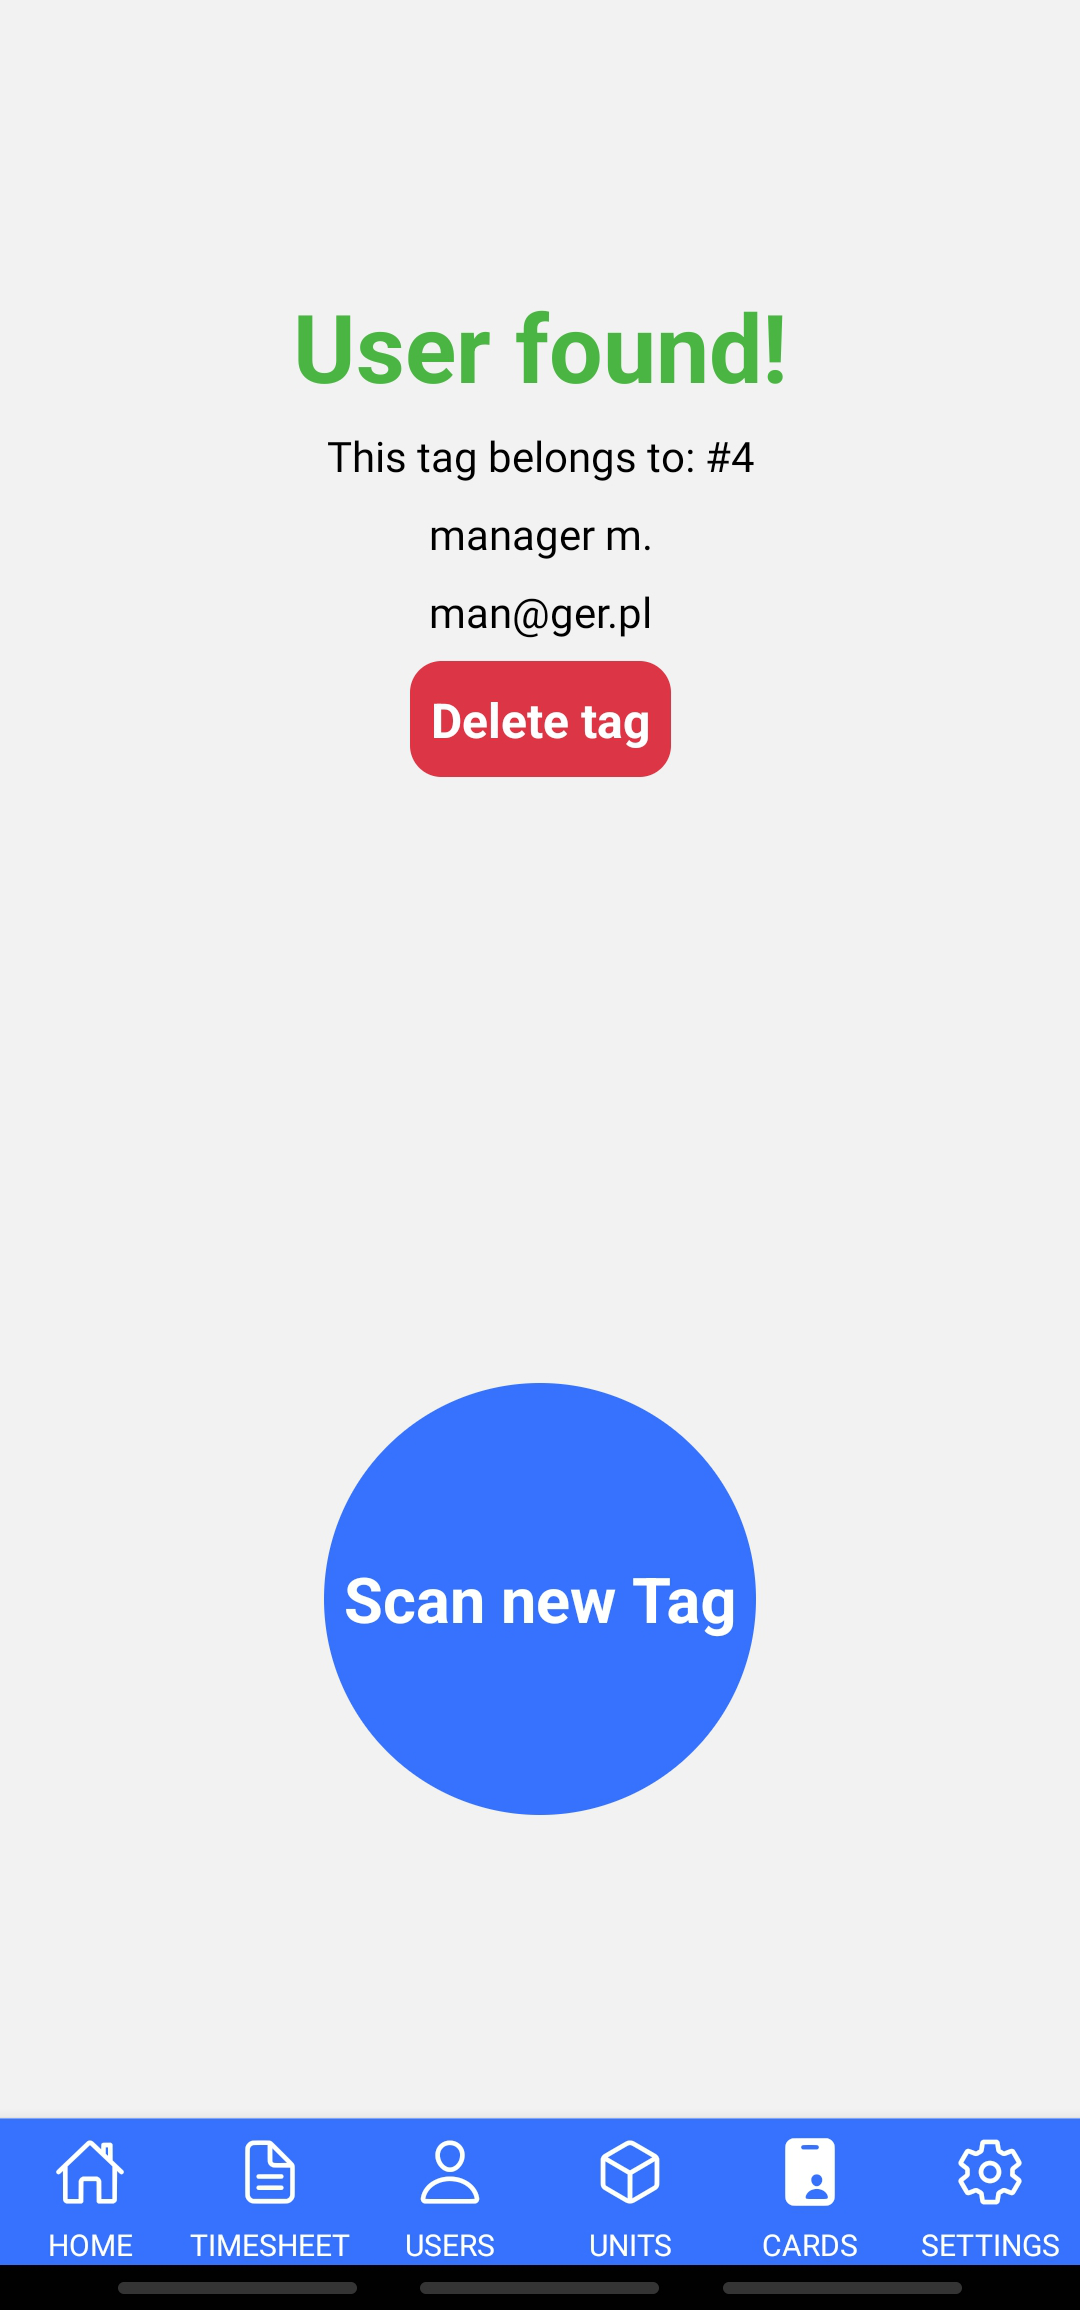
\includegraphics[width=\textwidth, frame]{graf/mobile/cardOwned.jpg}
        \caption{Karta przypisana}
    \end{subfigure}
    \begin{subfigure}[b]{0.3\textwidth}
        \centering
        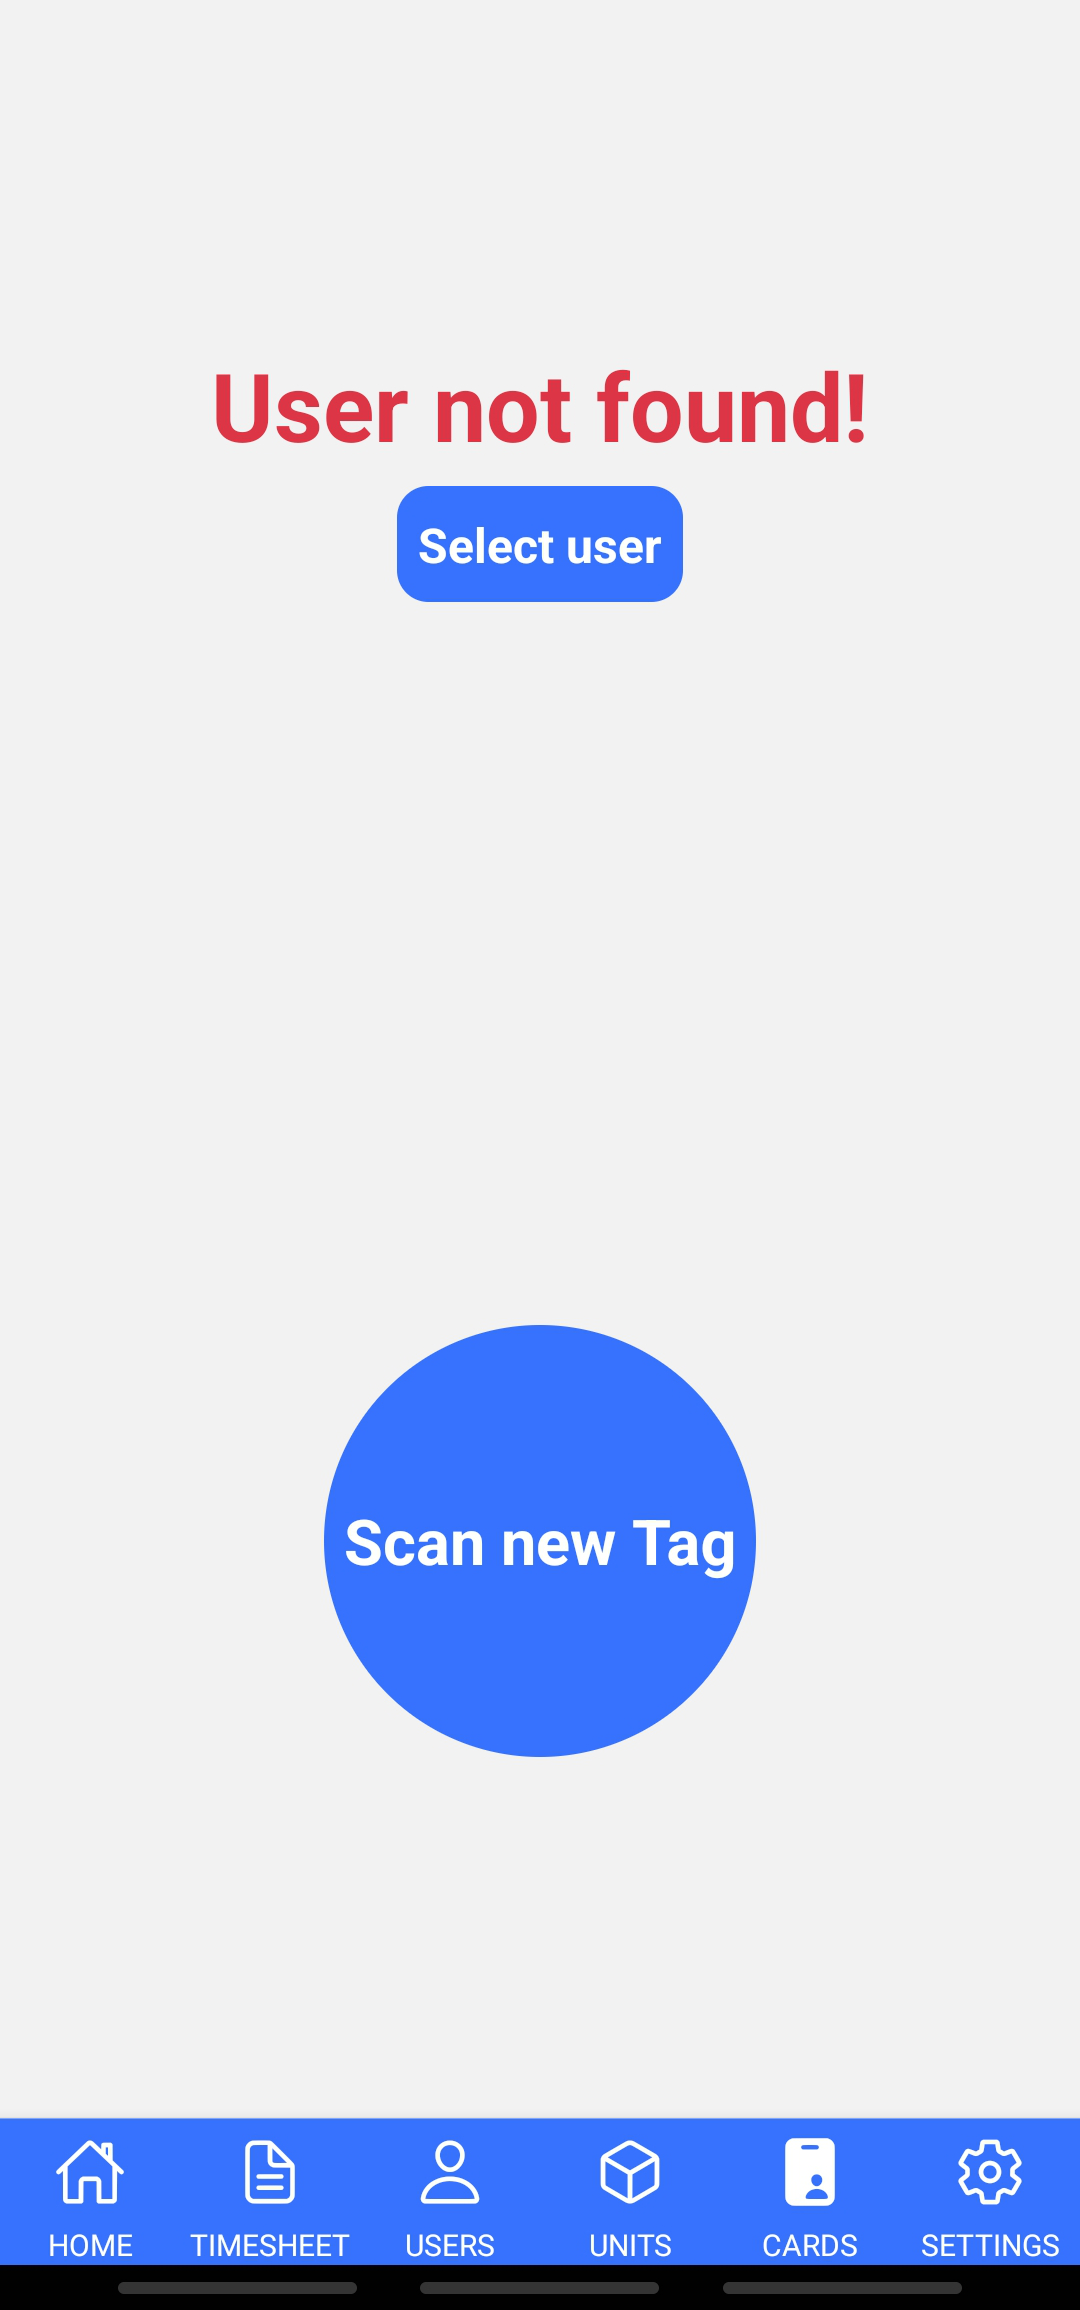
\includegraphics[width=\textwidth, frame]{graf/mobile/cardNotOwned.jpg}
        \caption{Karta nieprzypisana}
    \end{subfigure}
    \caption{Warianty widoku dodawania kart}
    \label{fig:cardView}
\end{figure}

Następnie - w zależności od wyniku zapytania - możliwe jest usunięcie karty z systemu lub przypisanie jej do użytkownika. W przypadku przypisania, administrator musi wybrać użytkownika z rozwijanej listy. Po zatwierdzeniu operacji, karta zostaje przypisana, a~administrator otrzymuje informację zwrotną o powodzeniu operacji. Widoki przypisania karty zostały przedstawione na rysunkach \ref{fig:cardDialogs}, a komunikat o powodzeniu operacji na~rysunku \ref{fig:cardSuccess}.

\begin{figure}
    \centering
    \begin{subfigure}[b]{0.3\textwidth}
        \centering
        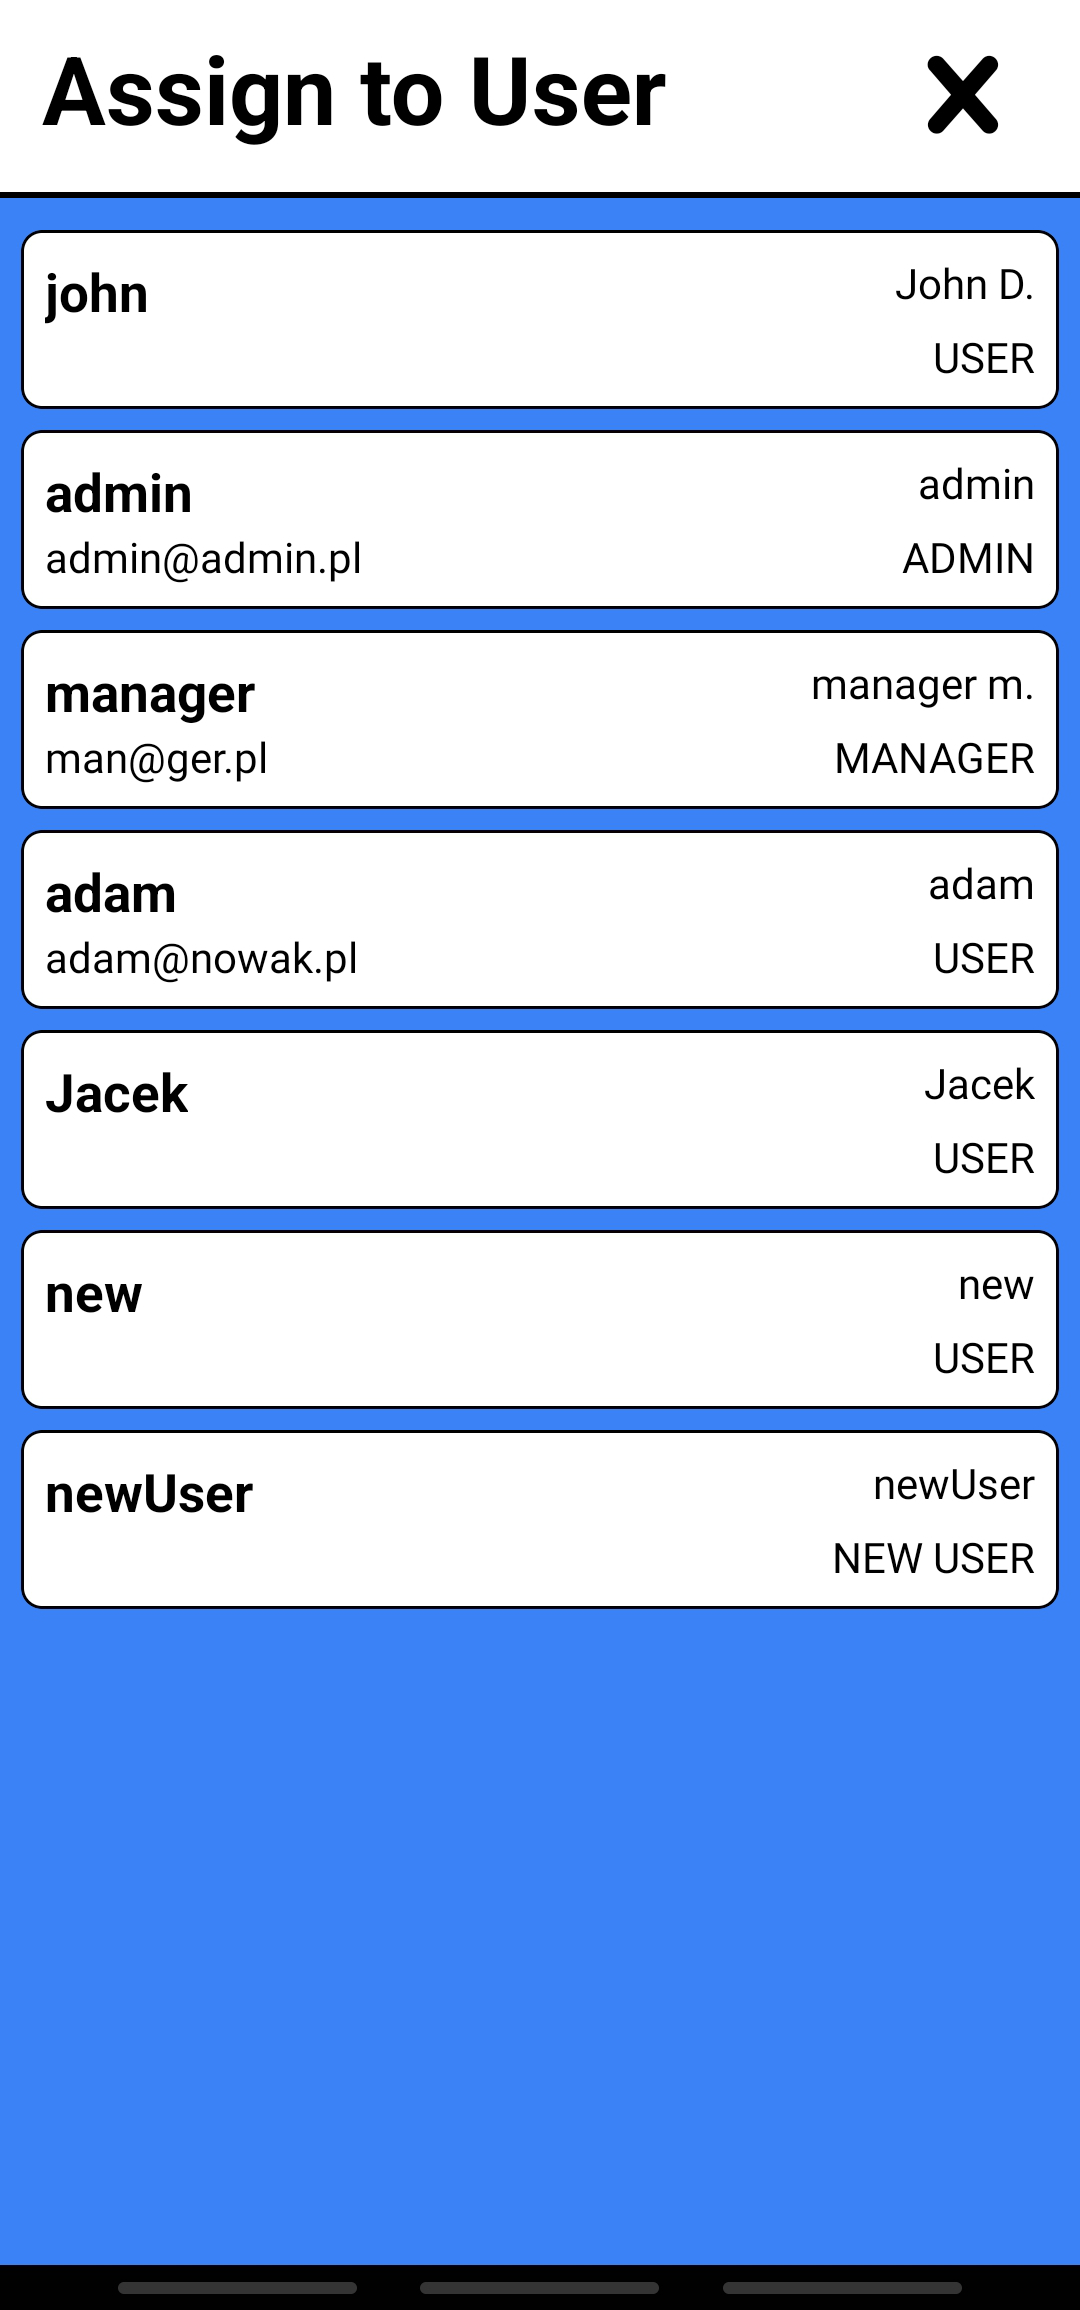
\includegraphics[width=0.8\textwidth, frame]{graf/mobile/userList.jpg}
        \caption{Lista użytkowników}
    \end{subfigure}
    \begin{subfigure}[b]{0.3\textwidth}
        \centering
        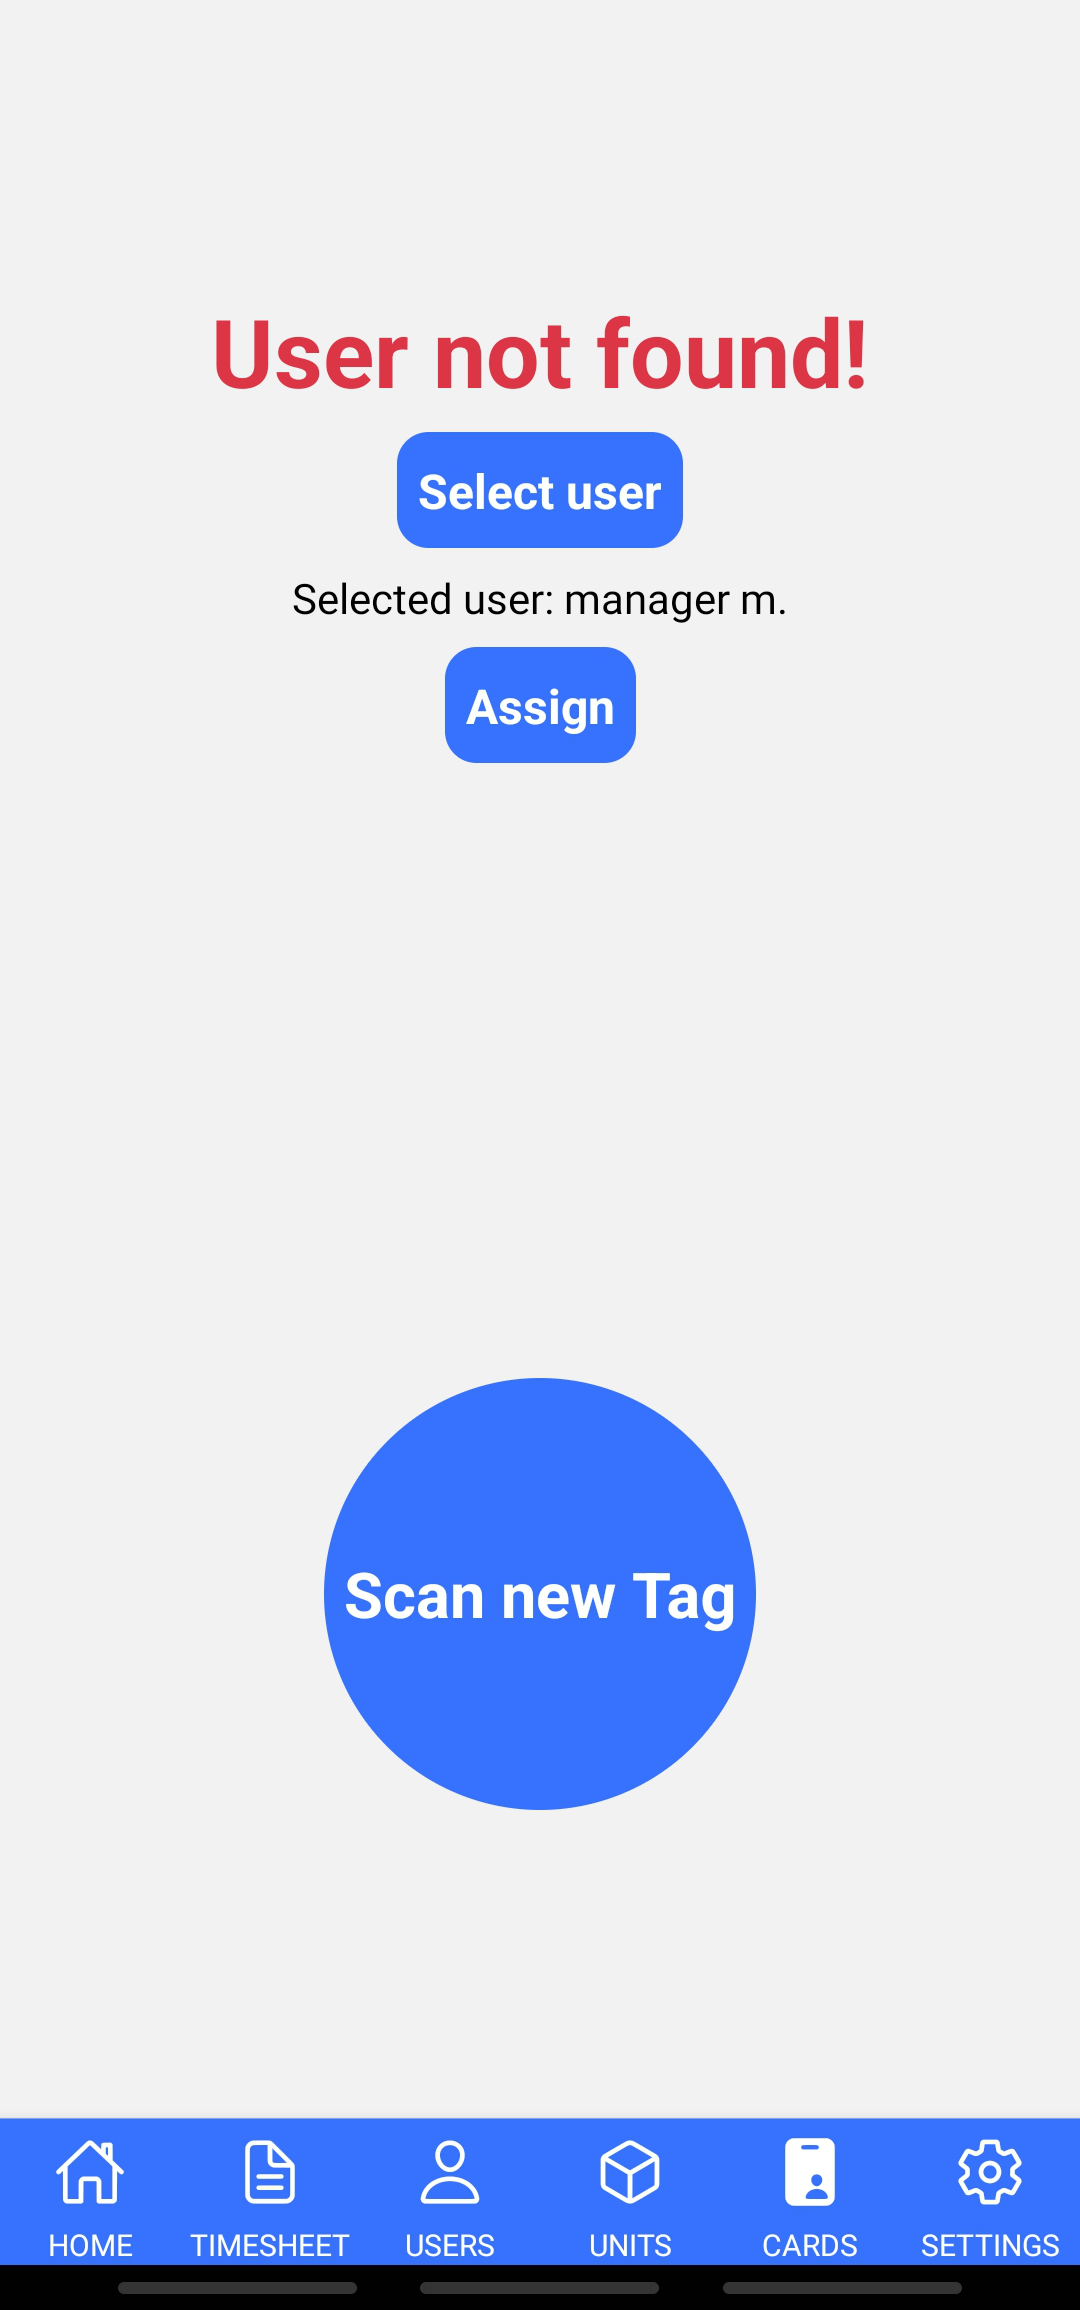
\includegraphics[width=0.8\textwidth, frame]{graf/mobile/userSelected.jpg}
        \caption{Wybrany użytkownik}
    \end{subfigure}
    \caption{Widoki dodawania kart}
    \label{fig:cardDialogs}
\end{figure}

\begin{figure}[H]
    \centering
    \begin{subfigure}[b]{0.49\textwidth}
        \centering
        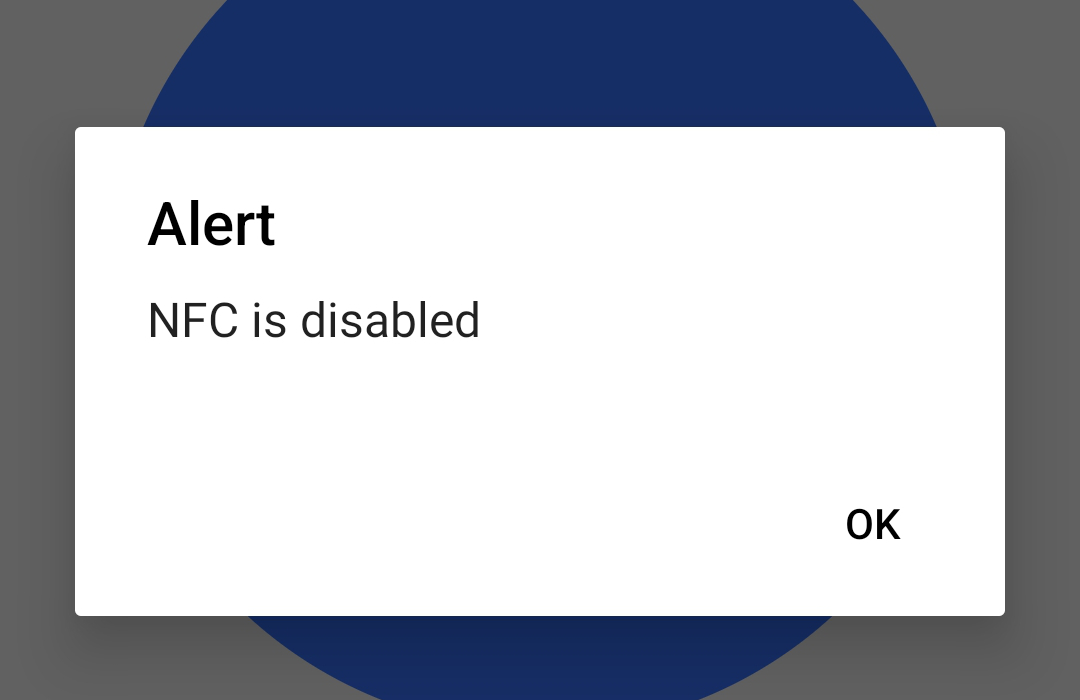
\includegraphics[width=0.7\textwidth, frame]{graf/mobile/nfcDisabled.jpg}
        \caption{Komunikat o konieczności włączenia NFC}
        \label{fig:cardNFC}
    \end{subfigure}
    \begin{subfigure}[b]{0.49\textwidth}
        \centering
        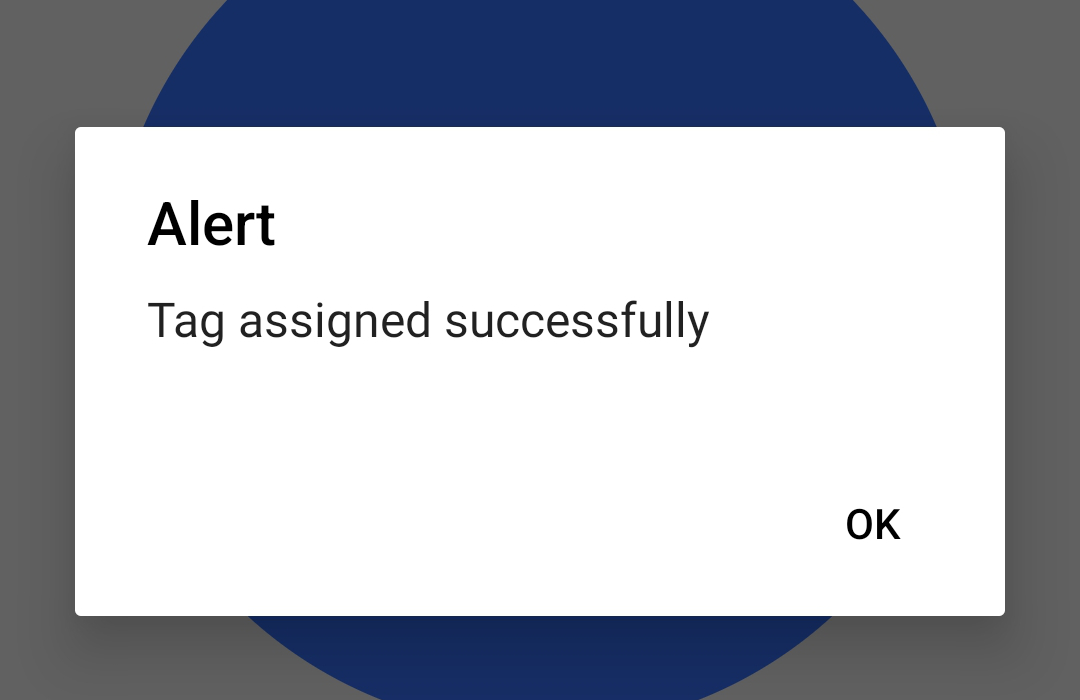
\includegraphics[width=0.7\textwidth, frame]{graf/mobile/success.jpg}
        \caption{Komunikat o powodzeniu operacji}
        \label{fig:cardSuccess}
    \end{subfigure}
    \caption{Komunikaty widoku dodawania kart}
\end{figure}

\section{Obsługa czytnika kart}

Czytnik kart jest prostym układem mikroprocesorowym, który kontaktuje się z serwerem w celu autoryzacji użytkowników.

\subsection{Uruchomienie}

Czytnik uruchamia się automatycznie po podłączeniu do zasilania. Podczas tego procesu dioda LED (ang. \english{Light Emitting Diode}) świeci się na żółto. Jeżeli czytnik napotka jakikolwiek problem podczas uruchamiania, dioda LED zmieni kolor na zielony, a~mikrokontroler udostępni sieć bezprzewodową, do której można się połączyć i otworzyć stronę konfiguracyjną. Widok strony konfiguracyjnej został przedstawiony na rysunku \ref{fig:readerConfig}.

\begin{figure}[H]
    \centering
    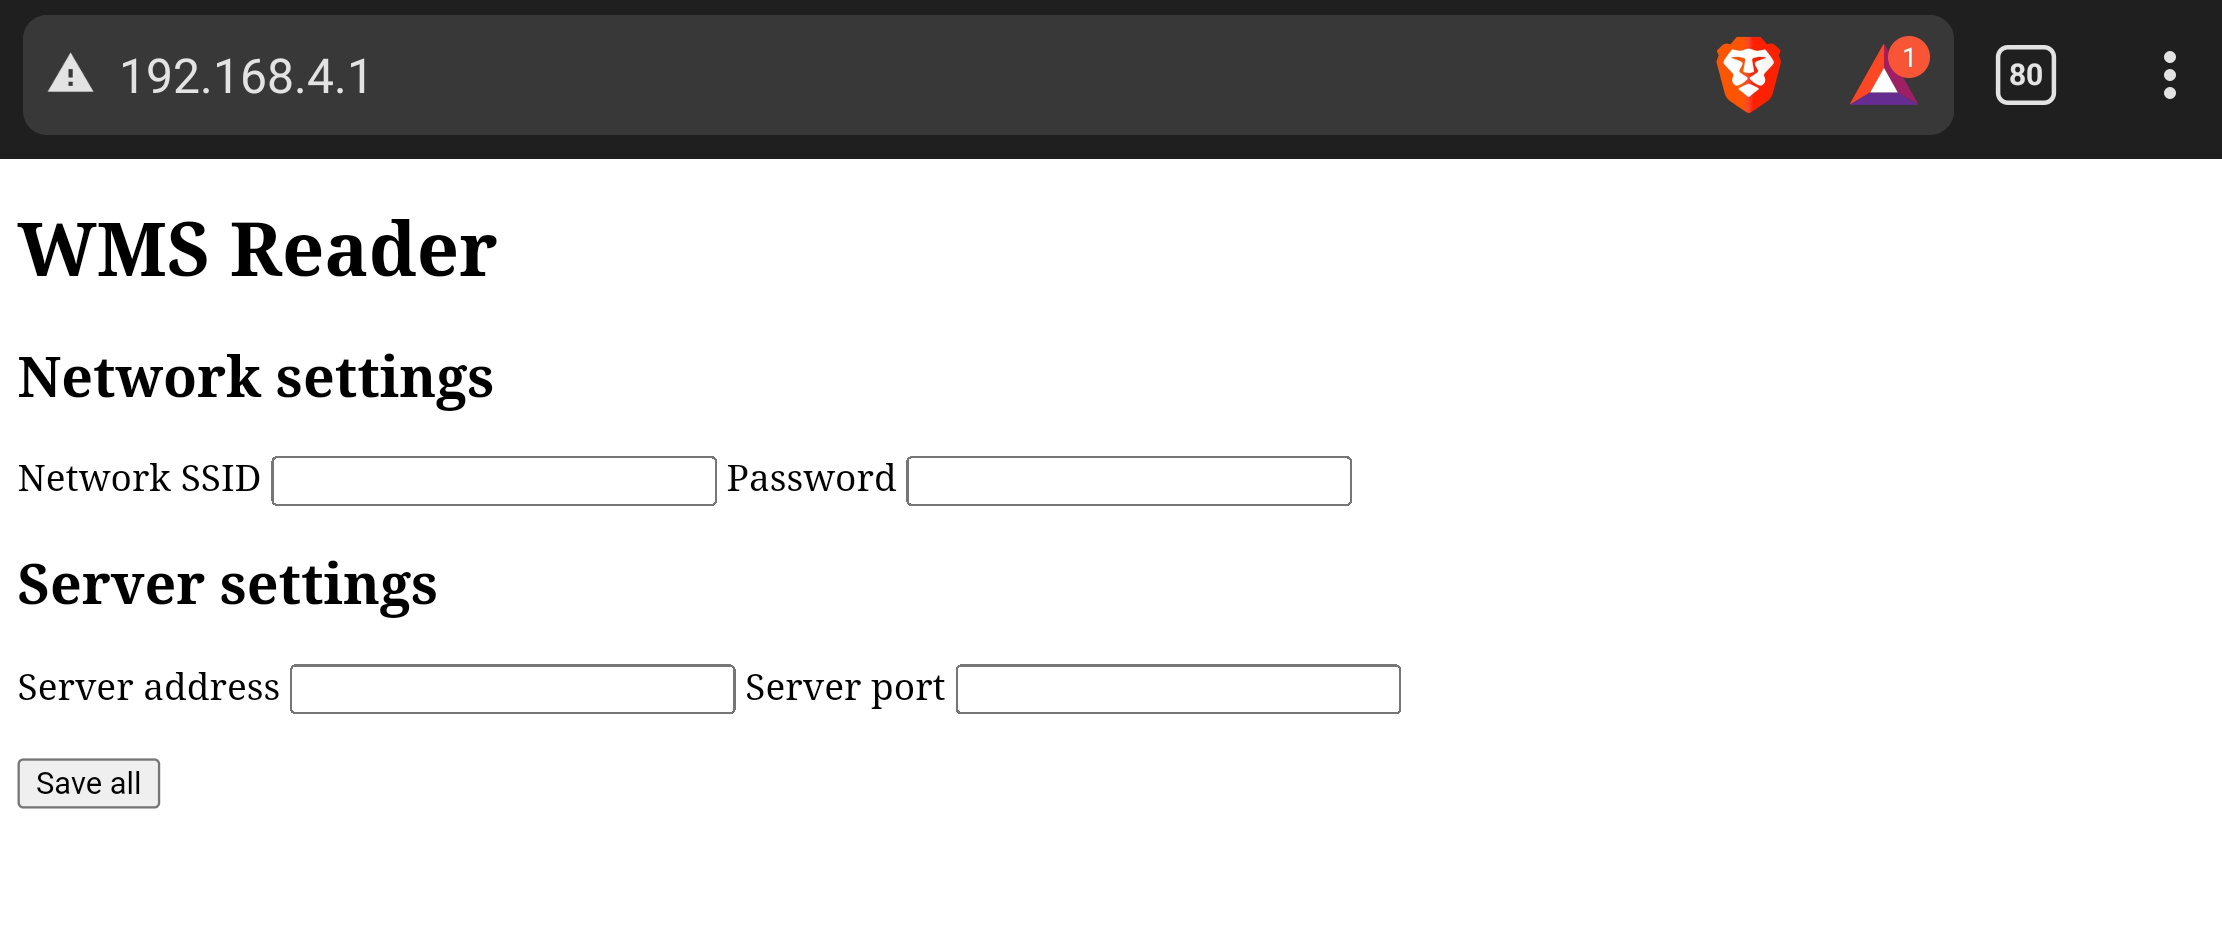
\includegraphics[width=0.7\textwidth, frame]{graf/readerSetup.jpg}
    \caption{Widok strony konfiguracyjnej czytnika.}
    \label{fig:readerConfig}
\end{figure}

Po poprawnym uruchomieniu, dioda LED zmienia kolor na niebieski.

\subsection{Odczyt karty}

Podczas normalnego trybu pracy czytnik oczekuje na zbliżenie karty. Po jej odczycie dioda LED zmienia kolor na żółty, kiedy to czytnik oczekuje na odpowiedź serwera. Następnie przez krótką chwilę świeci na zielono - jeśli odczyt się powiódł - lub na czerwono - jeśli wystąpił błąd. Po zakończeniu procesu, czytnik wraca do trybu oczekiwania na odczyt karty.

\section{Dostępność}

\subsection{Dostępność cyfrowa}

Aplikacja została zaprojektowana w taki sposób, aby możliwe było korzystanie z niej przy użyciu klawiatury. Użycie biblioteki komponentów \texttt{PrimeVue} pozwoliło na zapewnienie dostępności dla osób o ograniczeniach. Komponenty umieszczone na stronie internetowej są zgodne z wytycznymi \texttt{WCAG 2.1} \cite{bib:WCAG21}.

\subsection{Dostępność językowa}

W celu zapewnienia dostępności systemu użytkownikom z różnych krajów i regionów, aplikacja dostarcza możliwość zmiany języka interfejsu użytkownika. W chwili obecnej dostępne są 2 języki: polski i angielski, jednakże dodanie kolejnego nie wymaga od programisty dużego nakładu pracy. Każdy z języków jest przechowywany w oddzielnym pliku \texttt{.json}, co pozwala na jego łatwą modyfikację lub dodanie nowego. Część pliku zawierającego tłumaczenia na język polski została przedstawiona na listingu \ref{lst:pl}.

\begin{listing}[H]
    \begin{minted}[linenos,breaklines,frame=lines]{json}
"form": {
    "save": "Zapisz",
    "cancel": "Anuluj",
    "fieldRequired": "To pole jest wymagane",
    "invalidFormat": "Nieprawidłowy format"
},
\end{minted}
    \caption{Fragment pliku z tłumaczeniami na język polski}
    \label{lst:pl}
\end{listing}